\providecommand{\main}{../../main}
\documentclass[../../main/main.tex]{subfiles}


\begin{document}

\section{Setup characterisation and preliminary tests}
\label{sec:preliminary}

Before switching to the discussion of the acquisition and data analysis, we present the preliminary operations performed to characterise the apparatus. These are needed in order to improve the quality of the final measurements and to refine the analysis strategy as well as the approximations for a sufficiently simple but correct simulation. So, in this Section we discuss:
\begin{itemize}
    \item the characterisation of the SSB detector, including the meaningful information that can be extrapolated by the acquired waveforms in order to discriminate the background;
    \item the characterisation of ALPIDE detector, which constitutes a more delicate operation due to the kind of data acquired and to its working principles. In particular, a crucial aspect on which we will stress more attention is the X-ray background discrimination;
    \item the radioactive source characterisation, including the calculations to extrapolate the \( \alpha \) particle energy exiting from the gold protection foils, the uniformity of emission and the energy correlation with the angle of emission;
    \item before passing to the characterisation of the beam profile, we discuss a Python based numerical simulation through which we model the apparatus, the \( \alpha \) particles beam and the physics of scattering on the thin foils;
    \item lastly, we treat the beam characterisation by comparing the experimental data acquired without the scattering foil inserted in the relative support and the expectation obtained by the numerical simulation.
\end{itemize}



\subsection{SSB detector characterisation}

\paragraph{Waveform analysis strategy}
A first preliminary analysis is done by performing a test acquisition with the detector placed at an angular position of \( 0 \ \si{\deg} \) with respect to the beam line, setting the threshold trigger at \( 500 \ \si{mV} \) and with a time resolution of \( 12 \ \si{bits} \) and a sample rate of \( 200 \ \si{MS/s} \).
With this choice of sample parameters, each acquired waveform can be represented by a set of points \( (t_{i},y(t_{i})) \), with \( t_{i}=0,\dots,4999 \). An example is showed in \figref{fig:preliminary_ssb_waveform}, where the waveform has been smoothed with a moving average filter. As we can see:
\begin{itemize}
    \item the baseline of the signal spaces the region \( \mathcal{B} = \qty{t_{i} \lesssim 1000} \cup \qty{t_{i} \gtrsim 3000} \);
    \item the peak spaces the range \( \mathcal{P} = \qty{ 1000 \lesssim t_{i} \lesssim 3000} \).
\end{itemize}
Therefore, we calculate the baseline \( b \) with a simple average in the baseline region \( \mathcal{B} \). Now, knowing that the energy \( \mathcal{E} \) of the detected particle is proportional to the integral of the collected charge, we compute \( \mathcal{E} \) by simply integrating the waveform and subtracting the baseline:
\begin{equation}
    \mathcal{E}
    \propto
    \int_{t_{i}}^{t_{f}} Q(t) \mathrm{d}t
    \propto
    \sum_{i=i_{0}}^{i_{f}} y(t_{i}) - b(t_{f}-t_{0})
    \quad ,
    \label{eq:preliminary_ssb_baseline}
\end{equation}
where \( t_{f} = 4999 \) and \( t_{0} = 0 \). The histogram reporting the integrals for the test run is showed in \figref{fig:preliminary_ssb_integrals}.

Another important quantity that can be extracted from the waveforms, useful for background discrimination, is the amplitude in \( \si{mV} \). This can be easily estimated by subtracting the baseline \( b \) from \( \max\{ y_{i} \} \):
\begin{equation}
    \Delta V
    =
    \max\{ y(t_{i}) \} - b
    \quad .
    \label{eq:preliminary_ssb_amplitudes}
\end{equation}
We show the histogram for this quantity for the test run in \figref{fig:preliminary_ssb_amplitudes}.


\begin{figure*}[h]
    \begin{minipage}[c]{0.33\linewidth}
        \vspace{0pt}
        \centering
        \subfloat[Example of filtered waveform]{
            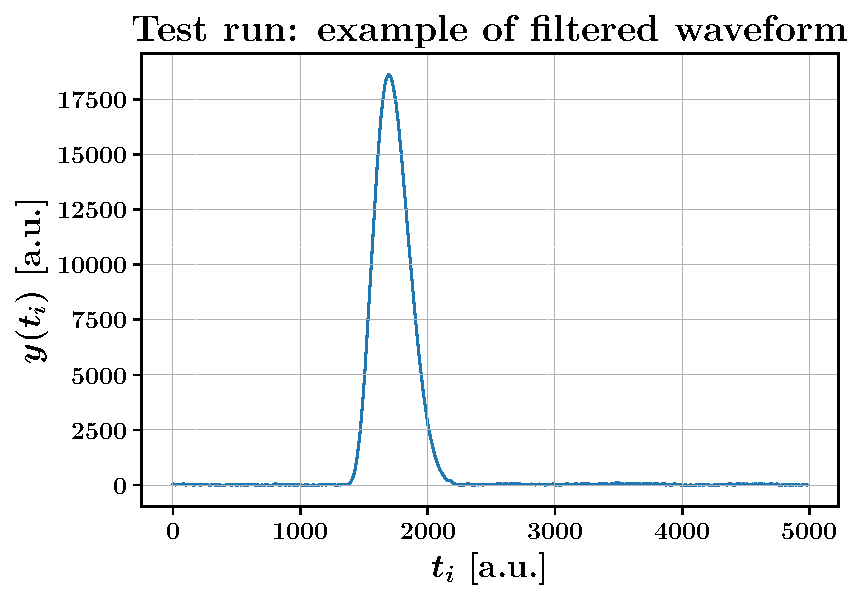
\includegraphics[height=4cm]{../sections/03/images/picoscope/test_run_waveform.pdf}
            \label{fig:preliminary_ssb_waveform}
        }
    \end{minipage}%
    \hfill%
    \begin{minipage}[c]{0.33\linewidth}
        \vspace{0pt}
        \centering
        \subfloat[Integral of waveforms]{
            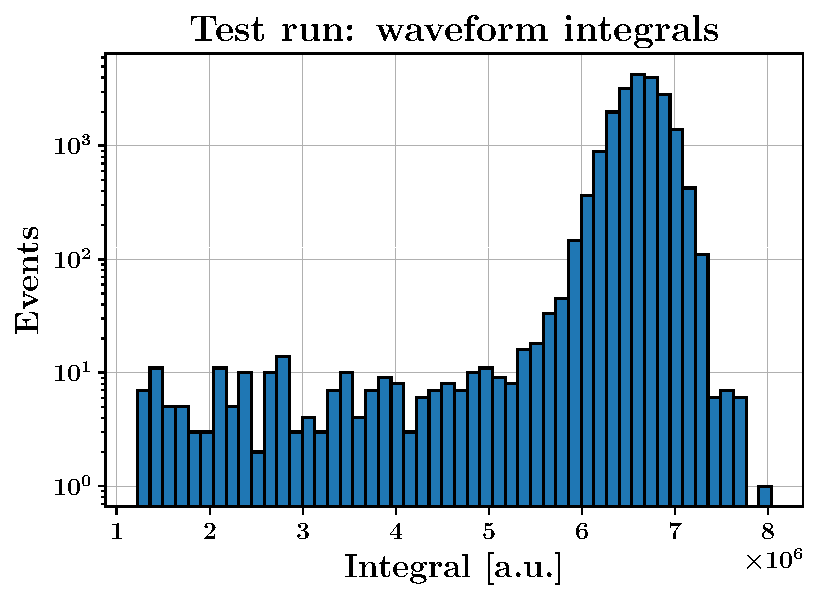
\includegraphics[height=4cm]{../sections/03/images/picoscope/test_run_integrals.pdf}
            \label{fig:preliminary_ssb_integrals}
        }
    \end{minipage}%
    \hfill%
    \begin{minipage}[c]{0.33\linewidth}
        \vspace{0pt}
        \centering
        \subfloat[Amplitudes of waveforms]{
            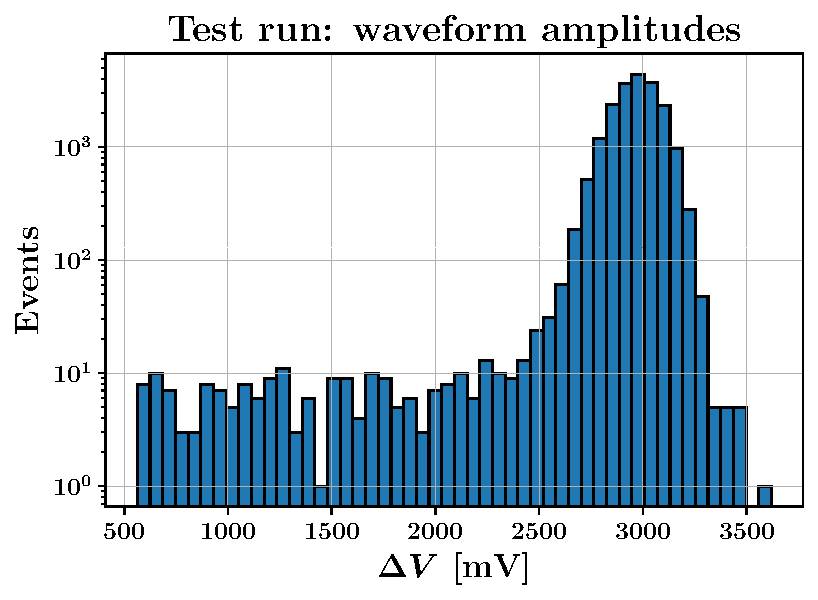
\includegraphics[height=4cm]{../sections/03/images/picoscope/test_run_amplitudes.pdf}
            \label{fig:preliminary_ssb_amplitudes}
        }
    \end{minipage}%
    \caption{Results for the test run and workflow for acquisitions with SSB detector. The filtered waveform shape is represented in \textbf{\ref{fig:preliminary_ssb_waveform}}, while the their integrals and amplitudes are showed in \textbf{\ref{fig:preliminary_ssb_integrals}} and \textbf{\ref{fig:preliminary_ssb_amplitudes}}, respectively.}
    \label{fig:preliminary_ssb_test_run}
\end{figure*}


\paragraph{Background discrimination strategy}
When dealing with low signal rates, namely when acquiring at a sufficiently large angular position with respect to the beam direction, it becomes of paramount importance to find an optimal strategy to discriminate the background events. This problem can be easily faced by measuring the rate of acquired events when the radioactive source is not inserted in the chamber. So, in this case the SSB will detect spurious events due to \( \alpha \)-decay from contaminants of the chamber or from cosmic rays.

During the experimental activities, we have performed about \( 74 \ \si{h} \) of background acquisition, leading to the spectra of integrals and amplitudes in \figref{fig:preliminary_ssb_bkg_integrals} and \figref{fig:preliminary_ssb_bkg_amplitudes}, respectively. Through an opportune visualisation of these results, we can notice how the background events are concentrated in a region after the amplitude value of \( 3500 \ \si{mV} \), which is outside of the signal region. So, the real background event rate when we select the events in the amplitude signal region, is lower than the one found by simply dividing the total events over the \( 74 \ \si{h} \) of acquisition by the total acquisition time.


\begin{figure*}[h]
    \begin{minipage}[c]{0.33\linewidth}
        \vspace{0pt}
        \centering
        \subfloat[Example of filtered waveform]{
            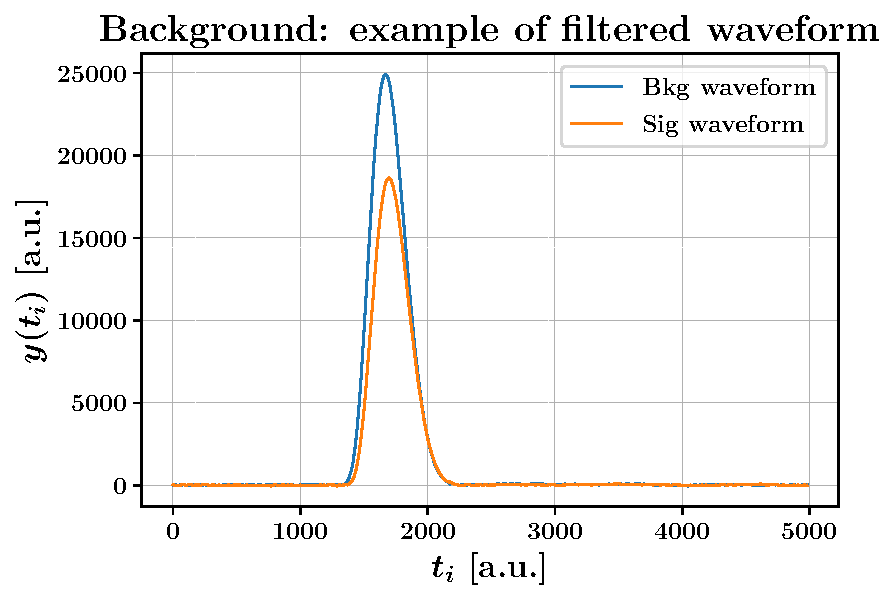
\includegraphics[height=4cm]{../sections/03/images/picoscope/bkg_run_waveform.pdf}
            \label{fig:preliminary_ssb_bkg_waveform}
        }
    \end{minipage}%
    \hfill%
    \begin{minipage}[c]{0.33\linewidth}
        \vspace{0pt}
        \centering
        \subfloat[Integral of waveforms]{
            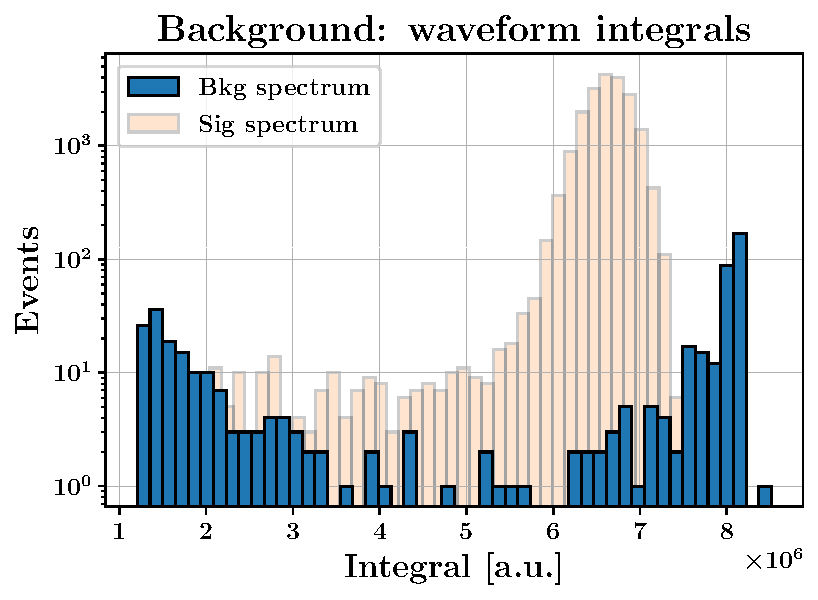
\includegraphics[height=4cm]{../sections/03/images/picoscope/bkg_run_integrals.pdf}
            \label{fig:preliminary_ssb_bkg_integrals}
        }
    \end{minipage}%
    \hfill%
    \begin{minipage}[c]{0.33\linewidth}
        \vspace{0pt}
        \centering
        \subfloat[Amplitudes of waveforms]{
            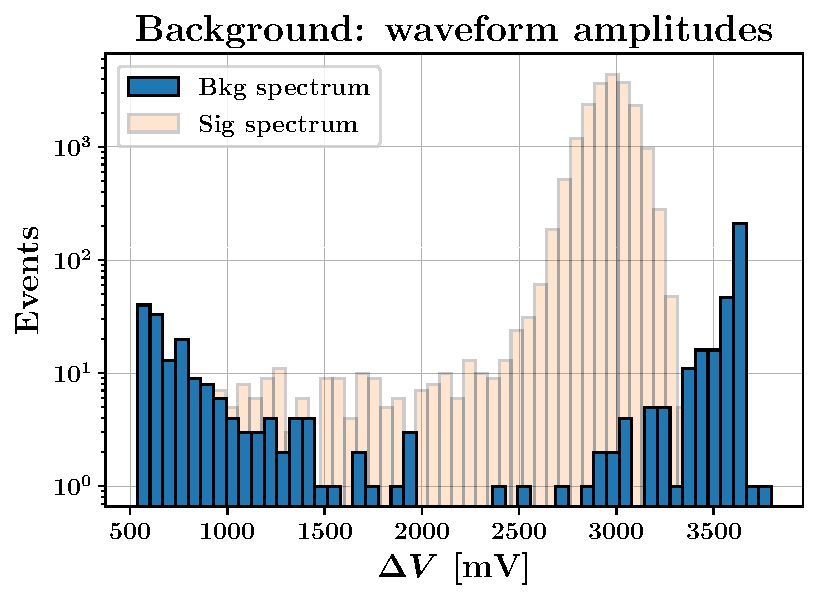
\includegraphics[height=4cm]{../sections/03/images/picoscope/bkg_run_amplitudes.pdf}
            \label{fig:preliminary_ssb_bkg_amplitudes}
        }
    \end{minipage}%
    \caption{Results for the run of background acquisition. A sample filtered waveform shape is showed in \textbf{\ref{fig:preliminary_ssb_bkg_waveform}} for both a signal and a background event. The spectra of integrals and amplitudes of all the events acquired are showed in \textbf{\ref{fig:preliminary_ssb_bkg_integrals}} and \textbf{\ref{fig:preliminary_ssb_bkg_amplitudes}}, respectively.}
    \label{fig:preliminary_ssb_bkg_run}
\end{figure*}




\paragraph{Dead time discussion}
Let us resume the discussion on the optimal choice of the number of segments in which we divide the memory of the PicoScope oscilloscope. This is an important and critical parameter when acquiring since it allows us to reduce the dead time contribution to the acquisition. Therefore, we choose a higher number of memory blocks when we expect higher rates, on the other hand we choose a lower one when we expect lower rates. However, even when an optimal choice can not be found, we can solve the problem by applying a correction on the total acquisition time. This is done by subtracting the sum of the time intervals in which the trigger is not active, but in a reset status. The ladder quantities can be retrieved from the timestamps provided by the acquisition system.



\subsection{ALPIDE detector characterisation}

\paragraph{Signal integrity analysis} The connection from the FPGA to APLIDE is made of 8 cables. Two of them are highly sensitive to external factors like noise introduced by the NIM electronics chain or the crosstalk between the cables.
Some precautions are applied to reduce these effects. Each sensible cable is wrapped with a ground lead. Moreover, they are placed away from other cables that may induce noise. On the other hand, an external power supply is used to power the FPGA board instead of powering it via USB. By this way, we are able to decouple the board from the PC supply systems\footnote{The various grounds (vacuum chamber, ALPIDE, SSB and PC systems) are not connected together}.

To verify the correct signal integrity a basic test can be used: a second FPGA (DE0-nano board equipped with a Cyclone IV by Altera \cite{DE0}) has the purpose to listen only to the continuous readout command and, after receiving it, a number sequence is sent and checked via software. If the sequence does not match, it will increase a counter and at the end of the test it gives the percentage of the corrupted data.

Many cable types have been tested during the experimental activity: jumper cables, flat ribbon cables, and modified cat 7 ethernet cable. The results of the previous test with each of them are reported in \tabref{tab:Cable}.


\begin{table}[!h]
    \centering
    \begin{tabular}{c|cccc}
        \toprule
        \textbf{Cable type}    & \textbf{Throughput$_{\mathrm{theo}}$ [Mbps]}   & \textbf{Throughput$_{\mathrm{exp}}$ [Mbps]}  &  \textbf{Time [h]}  & \textbf{Corrupted data [\%]}   \\
        \colrule
        Jumper            & $4.174$   & $4.120$   & 10  & $0$    \\
        Flat Ribbon Cable & $4.174$   & $0$       & 0.5 & FAILED \\
        Cat 7             & $4.174$   & $4.120$   & 10  & $0$    \\
        \botrule
    \end{tabular}
    \caption{Results of the test for signal integrity with several types of cable and comparison between them.}
    \label{tab:Cable}
\end{table}


\paragraph{Signal-to-noise discrimination}
Differently from the SSB detector, the ALPIDE detector is really sensitive to many sources of background, the main ones being cosmic rays, whose source is external to the experiment, and X-rays, produced by the radioactive source. It is therefore important to characterise the behaviour of the detector in order to discriminate these two from the \( \alpha \) particles.

The first study concerns the size and shape of the clusters generated on the detector from each type of radiation. This is accomplished by acquiring data in three different configurations of the radioactive source:
\begin{itemize}
    \item no source in the chamber: in this case we see only cosmic rays;
    \item shielded source: in this case we put the radioactive source in front of the detector but we cover its face with some layers of paper in order to stop the \( \alpha \) particles contribution but not the X-rays. With this configuration, we can acquire data about the full background;
    \item direct radiation: this last configuration is equal to the previous one minus the paper shield. In this case we obtain a sample with all the types of radiation.
\end{itemize}
To automatically detect the traces in each situation, we employ a clustering algorithm, chosen among the possibilities of DBSCAN and Agglomerative-Clustering, offered by the Scikit-Learn Python library.
A simple test to identify the best one shows how DBSCAN offers a better noise discrimination, hence it is chosen against the Agglomerative-Clustering method. Given this detail, we present some significant samples of hitmaps in \figref{fig:clust_hitmap}, where the several types of source and background radiations can be observed, while the pixel noise is rejected in both of them.


\begin{figure*}[h]
    \begin{minipage}[c]{0.49\linewidth}
        \vspace{0pt}
        \centering
        \subfloat[Actual hitmap (\( -63^{\circ} \))]{
            \includegraphics[width=\textwidth]{../sections/03/images/ALPIDE/ALPIDE_gold_alpide_53_SC_240m_run9_020121_hitmap.pdf}
            \label{fig:Big_Cosmic_hm}
        }
    \end{minipage}
    \hfill
    \begin{minipage}[c]{0.49\linewidth}
        \vspace{0pt}
        \centering
        \subfloat[Background hitmap (24h)]{
            \includegraphics[width=\textwidth]{../sections/03/images/ALPIDE/ALPIDE_bkg_24h_151220_hitmap.pdf}
            \label{fig:Bkg_hm}
        }
    \end{minipage}
    \caption{Sample hitmaps of the clusters revealed by ALPIDE detector. In \textbf{\ref{fig:Big_Cosmic_hm}}, an example of hitmap acquired at an angular position of \( -63^{\circ} \) with respect to the beam direction. In \textbf{\ref{fig:Bkg_hm}}, an example of hitmap from background acquisitions. The longer traces come from cosmic rays, while the bigger circular clusters are due to \( \alpha \) particles. Lastly, the smaller circular clusters are due to X-rays.}
    \label{fig:clust_hitmap}
\end{figure*}

The best parameters to identify the type of radiation are the size of the cluster and the ratio of the variance along the two main directions of the trace.
The ladder quantity is obtained by the application of a PCA algorithm to the cluster and finding the ratio between the variances along the main axes, namely the ``PCA ratio''. The results of this analysis are showed in \figref{fig:Area_histos} and \figref{fig:PCA_PCA_histos}. As we can see from these plots, the \( \alpha \) particles are characterised by big clusters: their area distribution presents a clear peak around \( 25 \) pixels, and small PCA ratios (\( \sim 1.5 \)). On the other hand, cosmic rays present very high PCA ratios and a wider area spectrum. Most cosmic rays have small areas (\( \sim 6 \) pixels) but, in some cases, the most energetic ones and the ones that are parallel to the detector surface are able to activate several dozens of pixels. Last but not least, the X-rays present an area distribution peaked to around \( 4 \) pixels.

\begin{figure*}[h]
    \begin{minipage}[c]{0.33\linewidth}
        \vspace{0pt}
        \centering
        \subfloat[Cosmic rays]{
            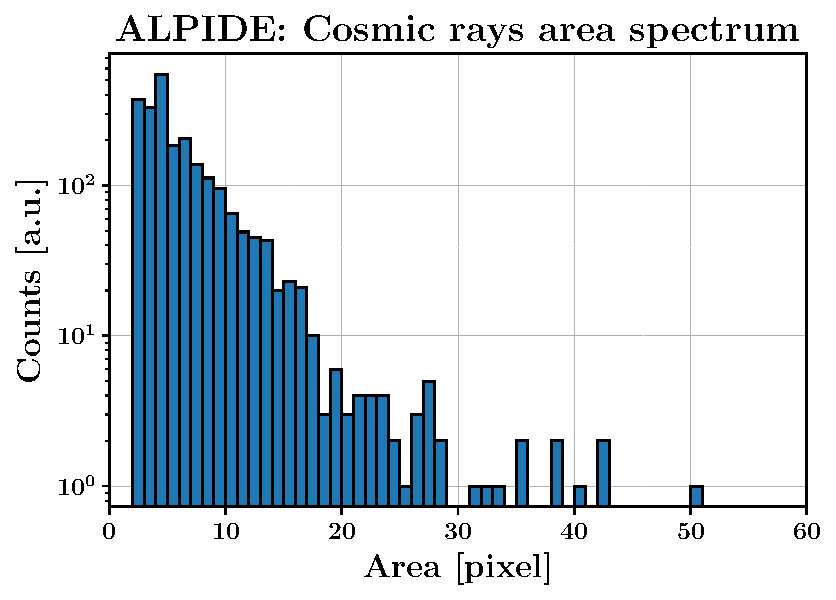
\includegraphics[height=4cm]{../sections/03/images/ALPIDE/ALPIDE_Cosmic_Area_hist_py.pdf}
            \label{fig:Cosmic_histo}
        }
    \end{minipage}%
    \hfill%
    \begin{minipage}[c]{0.33\linewidth}
        \vspace{0pt}
        \centering
        \subfloat[X and cosmic rays]{
            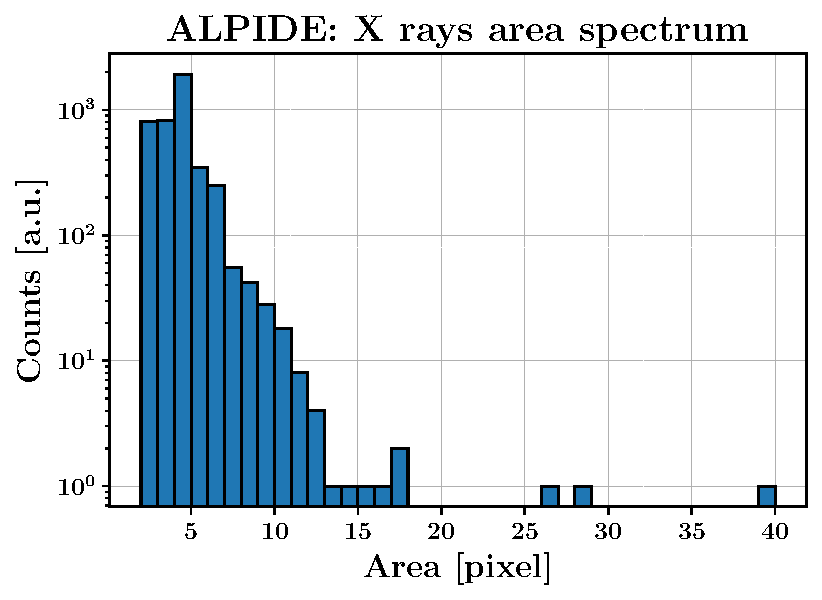
\includegraphics[height=4cm]{../sections/03/images/ALPIDE/ALPIDE_X_Area_hist_py.pdf}
            \label{fig:X_histo}
        }
    \end{minipage}%
    \hfill%
    \begin{minipage}[c]{0.33\linewidth}
        \vspace{0pt}
        \centering
        \subfloat[Compete area spectrum]{
            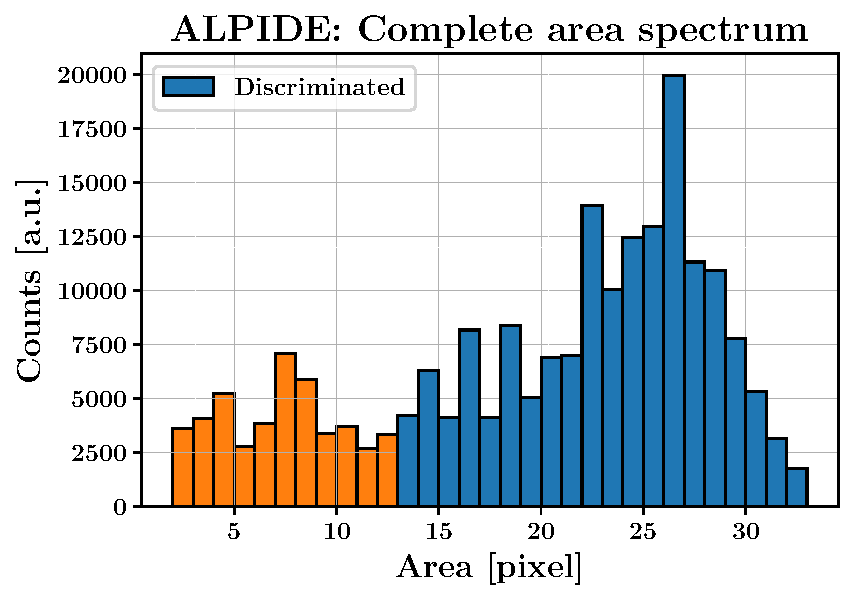
\includegraphics[height=4cm]{../sections/03/images/ALPIDE/ALPIDE_Alpha_Area_hist_py.pdf}
            \label{fig:Alpha_histo}
        }
    \end{minipage}
    \caption{Size of the cluster induced by different types of radiation on the ALPIDE detector. In \textbf{\ref{fig:Cosmic_histo}}, the distribution for cosmic rays, while in \textbf{\ref{fig:X_histo}} the distribution for both X and cosmic rays. Lastly, in \textbf{\ref{fig:Alpha_histo}}, the discriminated \( \alpha \) particles distribution in the complete area distribution.}
    \label{fig:Area_histos}
\end{figure*}


\begin{figure*}[h]
    \begin{minipage}[c]{0.33\linewidth}
        \vspace{0pt}
        \centering
        \subfloat[Cosmic rays]{
            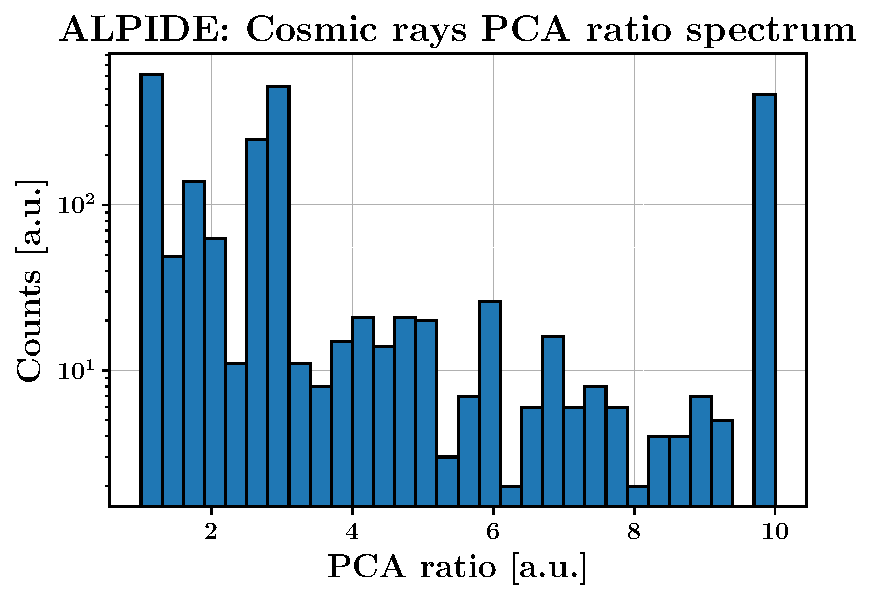
\includegraphics[height=4cm]{../sections/03/images/ALPIDE/ALPIDE_Cosmic_PCA_hist_py.pdf}
            \label{fig:Cosmic_PCA_histo}
        }
    \end{minipage}%
    \hfill%
    \begin{minipage}[c]{0.33\linewidth}
        \vspace{0pt}
        \centering
        \subfloat[X and cosmic rays]{
            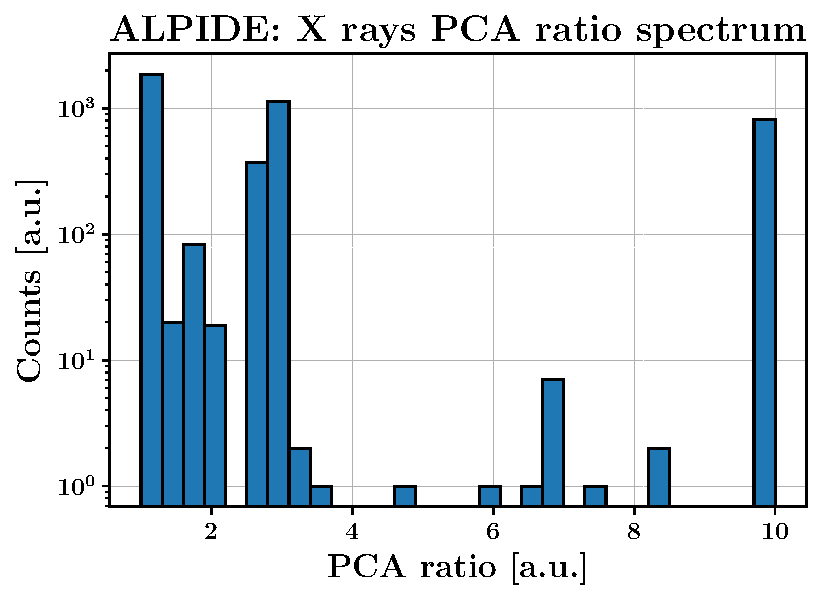
\includegraphics[height=4cm]{../sections/03/images/ALPIDE/ALPIDE_X_PCA_hist_py.pdf}
            \label{fig:X_PCA_histo}
        }
    \end{minipage}%
    \hfill%
    \begin{minipage}[c]{0.33\linewidth}
        \vspace{0pt}
        \centering
        \subfloat[Complete PCA ratio spectrum]{
            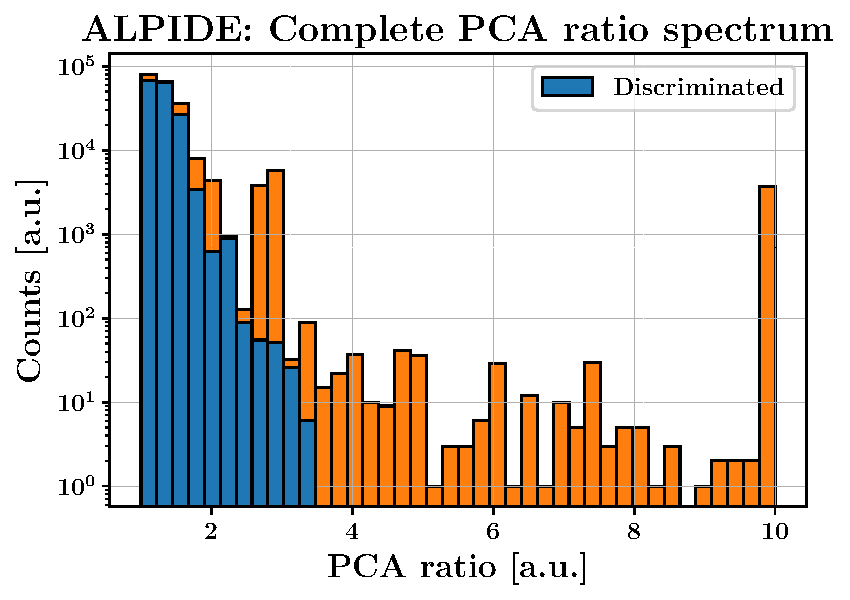
\includegraphics[height=4cm]{../sections/03/images/ALPIDE/ALPIDE_Alpha_PCA_hist_py.pdf}
            \label{fig:Alpha_PCA_histo}
        }
    \end{minipage}
    \caption{Ratio between the variance on the two main cluster components computed with a PCA algorithm for different types of radiation on the ALPIDE detector. In \textbf{\ref{fig:Cosmic_PCA_histo}}, the PCA ratio for cosmic rays, while in \textbf{\ref{fig:X_PCA_histo}} the PCA ratio for both X and cosmic rays. Lastly, in \textbf{\ref{fig:Alpha_PCA_histo}}, the discriminated \( \alpha \) particles PCA ratio in the complete distribution.}
    \label{fig:PCA_PCA_histos}
\end{figure*}


We report the mean values of the cluster area and PCA ratio for all the types of radiation in \tabref{tab:clust_features}.
Using this information, we can statistically discriminate signal events from background ones by considering only clusters with area \( A > 12 \) and PCA ratio \( P_{\mathrm{r}} < 3.5 \). In the same table we report also the mean values for a discriminated set of clusters, indicated with the notation \( \alpha_{\mathrm{disc}} \). As we can see, the mean area increases and it is very close to the peak value of \( 25 \) pixels observed in \figref{fig:Alpha_histo}.

\begin{table}[!h]
    \centering
    \begin{tabular}{c|ccc}
        \toprule
        \textbf{Particle} & \textbf{Area [pixel]}    & \textbf{PCA ratio} & \textbf{Rate [ev/h]}    \\
        \colrule
        Cosmic rays         & $6.0\pm6.3$   & $3.9\pm3.3$ & $5.79 \cdot 10^{2}$  \\
        X rays              & $3.8\pm1.6$   & $3.4\pm3.3$ & $2.88 \cdot 10^{4}$ \\
        $\alpha$            & $19.5\pm8.0$  & $1.6\pm1.2$ & $1.46 \cdot 10^{6}$ \\
        $\alpha_{\mathrm{disc}}$     & $23.0\pm4.8$  & $1.3\pm0.2$ & $1.15 \cdot 10^{6}$ \\
        \botrule
    \end{tabular}
    \caption{Summary of the main cluster features for different types of radiation and for a discriminated sample \( \alpha_{\mathrm{disc}} \).}
    \label{tab:clust_features}
\end{table}


\paragraph{Threshold analysis}
The threshold at which the pixel fires when a particle traverses is mainly set by the $I_{\mathrm{THR}}$ and $V_{\mathrm{CASN}}$ values \cite{Manual_ALP}.
These parameters can be modified by writing the DAC value on a given register \cite{Manual_ALP}, which has 8 bit resolution and sweeps from AVSS (equal to \( 0 \ \si{V} \)) to AVDD (equal \( 1.8 \ \si{V} \))\footnote{Some DACs have a unitary gain buffer which introduces an offset of \( 370 \ \si{mV} \); $V_{\mathrm{CASN}}$ is not one of them, in fact it is directly connected to the pixel matrix.}.
The charge threshold is decreased by augmenting $V_{\mathrm{CASN}}$ and vice versa, it is increased by increasing $I_{\mathrm{THR}}$.

In our studies, $V_{\mathrm{CASN}}$ is the only parameter modified (register \texttt{0x0604}). We report in \figref{fig:THR_graph} the results of some tests performed to find the optimal value of $V_{\mathrm{CASN}}$, in order to maximise the discrimination power of our methods to distinguish between X-rays, cosmic rays and $\alpha$-particles.


\begin{figure*}[h]
    \begin{minipage}[c]{0.33\linewidth}
        \vspace{0pt}
        \centering
        \subfloat[Area vs $V_{\mathrm{CASN}}$]{
            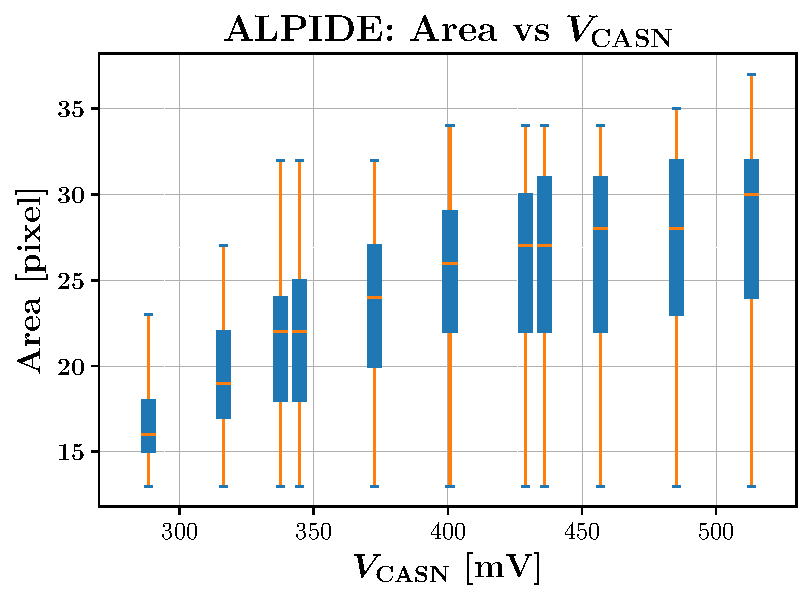
\includegraphics[height=4cm]{../sections/03/images/ALPIDE/ALPIDE_Area_graph_py_box.pdf}
            \label{fig:THR_area}
        }
    \end{minipage}%
    \hfill%
    \begin{minipage}[c]{0.33\linewidth}
        \vspace{0pt}
        \centering
        \subfloat[PCA ratio vs $V_{\mathrm{CASN}}$]{
            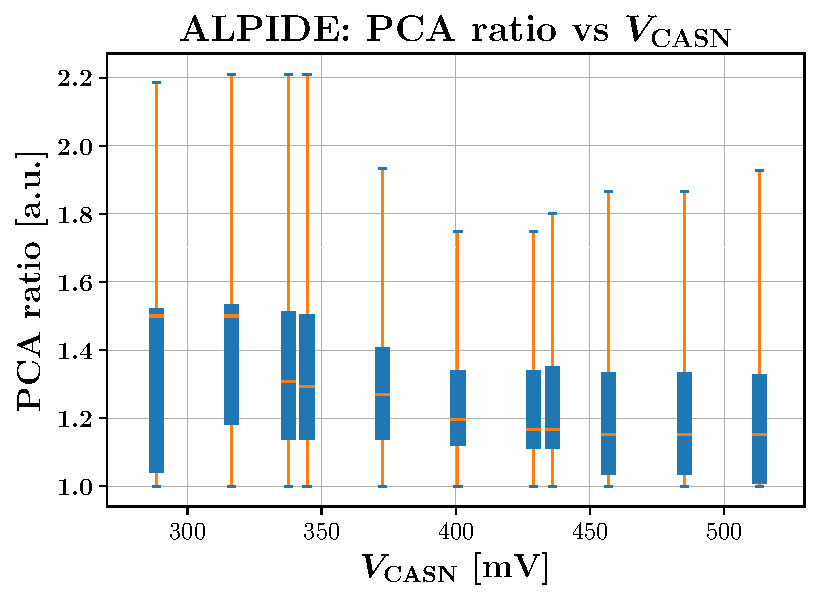
\includegraphics[height=4cm]{../sections/03/images/ALPIDE/ALPIDE_PCAr_graph_py_box.pdf}
            \label{fig:THR_PCA}
        }
    \end{minipage}%
    \hfill%
    \begin{minipage}[c]{0.33\linewidth}
        \vspace{0pt}
        \centering
        \subfloat[SNR vs $V_{\mathrm{CASN}}$]{
            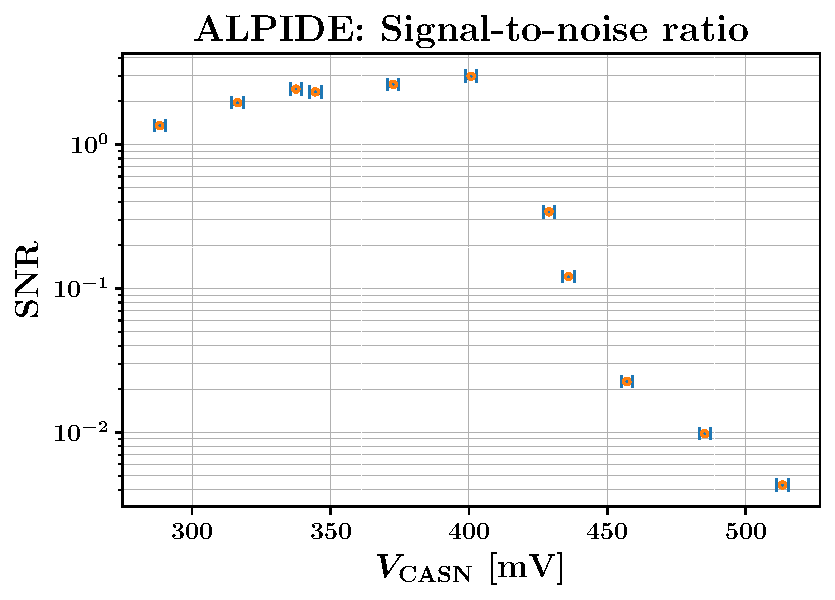
\includegraphics[height=4cm]{../sections/03/images/ALPIDE/ALPIDE_SNR_graph_py.pdf}
            \label{fig:THR_SNR}
        }
    \end{minipage}
    \caption{Results for \( V_{\mathrm{CASN}} \) parameter optimisation. In particular, in \textbf{\ref{fig:THR_area}}, \textbf{\ref{fig:THR_PCA}} and \textbf{\ref{fig:THR_SNR}} the Area of clusters, the PCA ratio and the SNR in function of \( V_{\mathrm{CASN}} \), respectively.}
    \label{fig:THR_graph}
\end{figure*}


Firstly a simple software threshold is set to discard X-rays and eventual cosmic rays\footnote{This software threshold is tuned once the optimal $V_{\mathrm{CASN}}$ is chosen.}, so that only clusters with area above 12 pixels and PCA ratio below 4 are considered. A higher value of the mean area threshold leads to a better discrimination between unwanted particles. As it showed in \figref{fig:THR_area}, the dependence on $V_{\mathrm{CASN}}$ becomes weaker at higher values.

In \figref{fig:THR_PCA} we highlight how the PCA ratio dispersion has a minimum around $V_{\mathrm{CASN}} = 400 \ \si{mV}$, with higher values for lower $V_{\mathrm{CASN}}$. It is clear from \figref{fig:THR_SNR} that going beyond \( 400 \ \si{mV} \) implies a lower SNR and considering the readout limitations introduced above, a value of \( 373 \ \si{mV} \) is selected (corresponding to a value of \texttt{0x0035} on the register). This value of $V_{\mathrm{CASN}}$ gives us the best compromise between particle discrimination and acquirable rate.


\paragraph{Timing analysis}
As we have highlighted in the previous discussion, due to the limitations introduced by the slow port, it necessary to make some compromises on the readout speed. This is accomplished by tuning the time fraction in which the detector can store the data, namely the so-called \textbf{STROBE}, and the gap between two subsequent trigger signals, namely the so-called \textbf{GAP}, both expressed in units of clock cycles.
We observe that if the strobe time is too low, the charge produced by the $\alpha$ particles can not be completely collected and therefore the discrimination from the X-rays is problematic. So, a value of 5000 clock cycles is selected\footnote{{Corresponding to 125 $\mu s$}} to avoid this drawback.

To avoid the FIFO overflow, the gap needs to be tuned for each case. For small angles where the expected rate is higher, a larger gap value is set, while for higher angles a lower gap is selected due to the lower statistics.
The effective exposition time \( t_{\mathrm{exp}} \) of ALPIDE will follow the expression:
\begin{equation}
    t_{\mathrm{exp}}
    =
    t_{\mathrm{acq}} r
    =
    t_{\mathrm{acq}} \frac{t_{\mathrm{strobe}}}{t_{\mathrm{strobe}} + t_{\mathrm{gap}}}
    \quad .
    \label{eq:alpide_strobe_gap}
\end{equation}
A test to verify the linearity of the effective exposition time in \eqnref{eq:alpide_strobe_gap} can be performed.
With this purpose, the radioactive source is placed at a fixed distance from ALPIDE and an acquisition is launched for different values of strobe and gap, with an acquisition time of \( 60 \ \si{s} \), and then measuring the rate. A plot with the results of this study is showed in \figref{fig:strobe_analysis}, where we perform also a linear fit to verify the linear trend of the rate with respect to the ratio \( r \) of strobe and strobe plus gap.


\begin{figure*}[h]
    \begin{minipage}[c]{0.49\linewidth}
        \vspace{0pt}
        \centering
        \subfloat[Plot of measurements, fit and residuals]{
            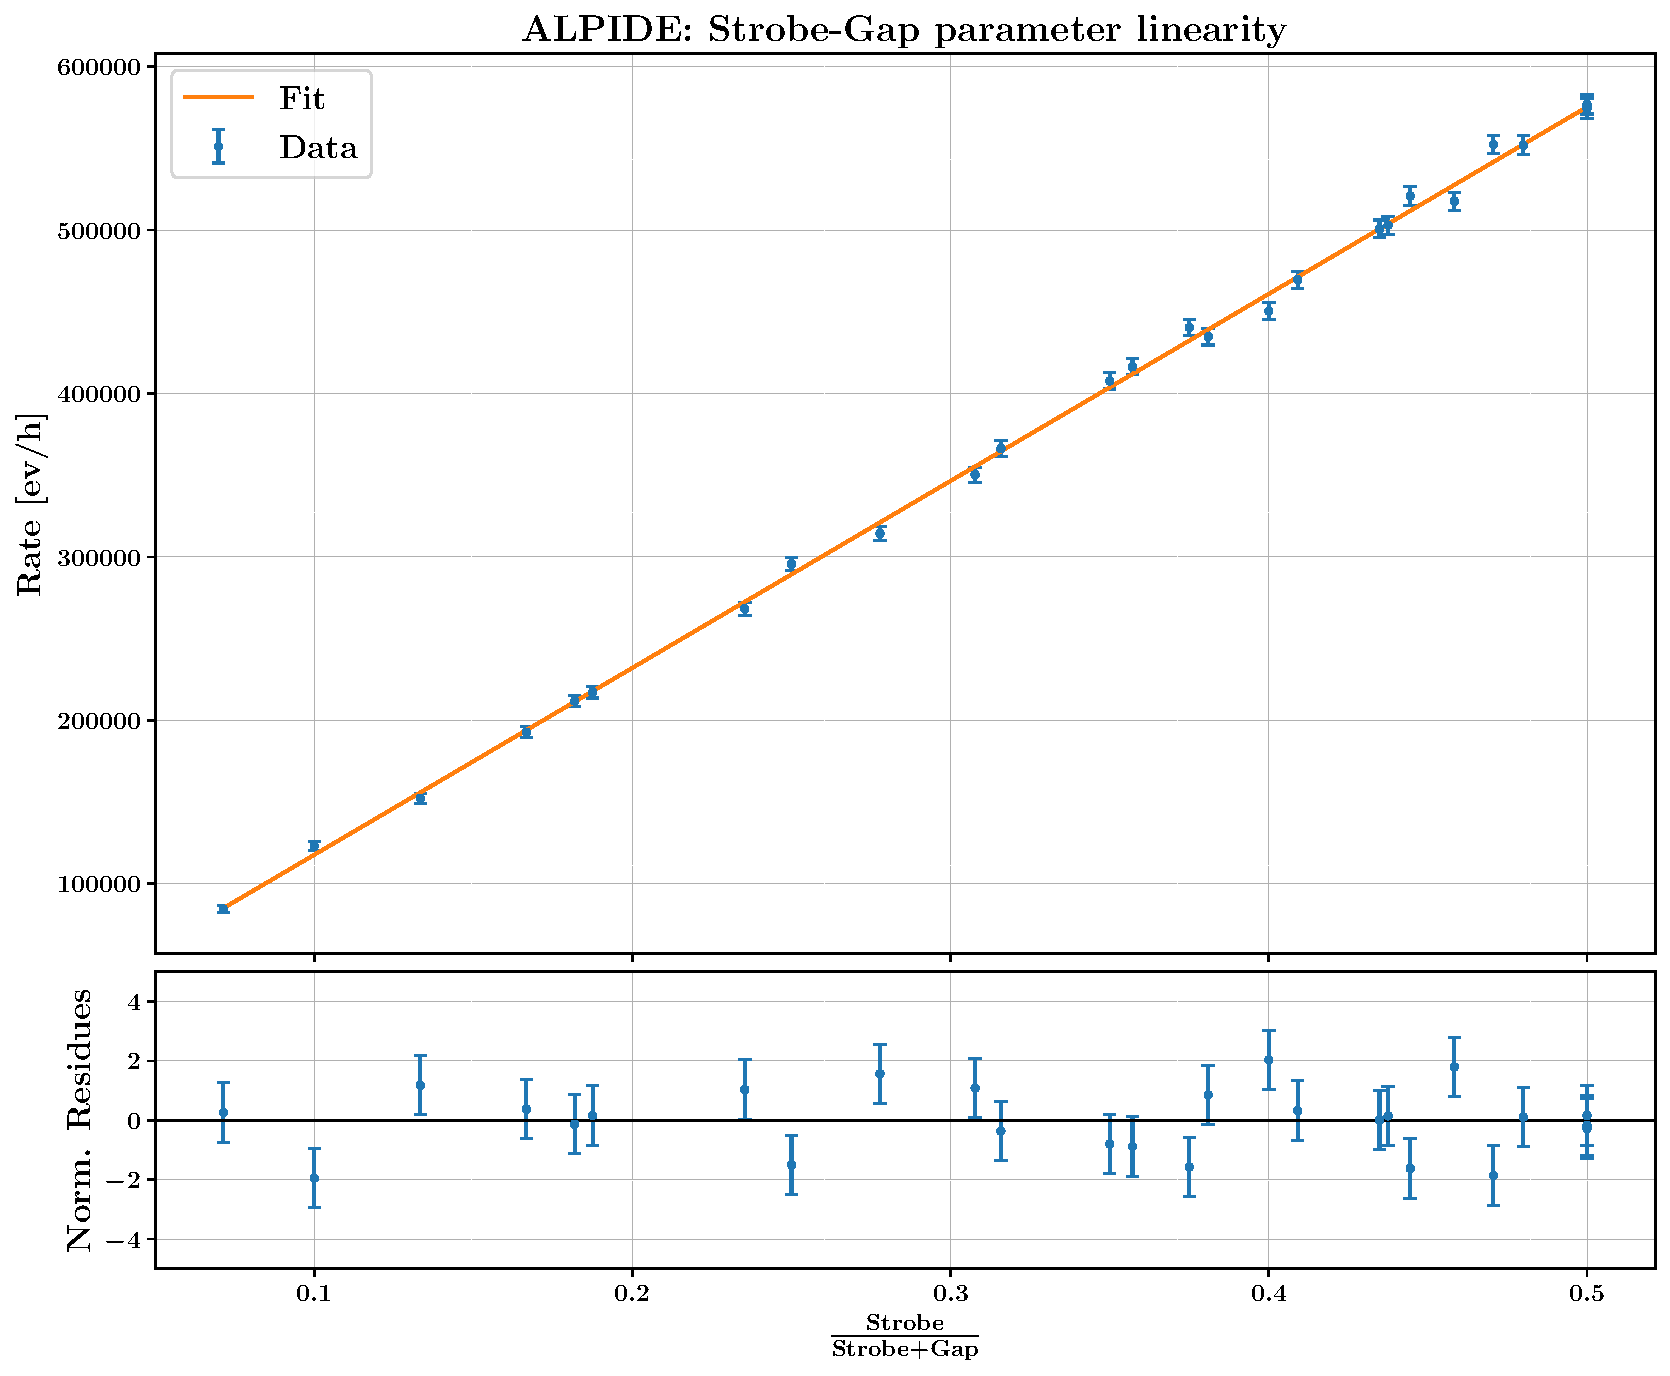
\includegraphics[width=1.0\linewidth, valign=c]{../sections/03/images/ALPIDE/ALPIDE_str_par.pdf}
            \label{fig:strobe_plot}
        }
    \end{minipage}%
    \hfill%
    \begin{minipage}[c]{0.49\linewidth}
        \vspace{0pt}
        \centering
        \subfloat[Measurements and fit results]{
            \adjustbox{valign=c}{
            {\scriptsize
                \begin{tabular}{ccc|ccc}
                    \toprule
                    \multicolumn{6}{c}{\textbf{Data}}   \\
                    \colrule
                    \textbf{Strobe} & 
                    \textbf{Gap} & 
                    \textbf{Rate} &
                    \textbf{Strobe} & 
                    \textbf{Gap} & 
                    \textbf{Rate} \\
                    \textbf{cycles} & 
                    \textbf{cycles} & 
                    \textbf{[$\boldsymbol{10^3}\cdot$ ev/h]} &
                    \textbf{cycles} & 
                    \textbf{cycles} & 
                    \textbf{[$\boldsymbol{10^3}\cdot$ ev/h]} \\
                    \colrule
                    20000 &	45000 & 350 $\pm$ 5  & 35000 &	45000 & 503 $\pm$ 5 \\
                    45000 &	45000 & 574 $\pm$ 6  & 30000 &	45000 & 450 $\pm$ 5 \\
                    30000 &	65000 & 366 $\pm$ 5  & 50000 &	65000 & 501 $\pm$ 5 \\
                    60000 &	65000 & 552 $\pm$ 6  & 25000 &	25000 & 577 $\pm$ 6 \\
                    40000 &	65000 & 435 $\pm$ 5  & 25000 &	65000 & 314 $\pm$ 4 \\
                    20000 &	25000 & 521 $\pm$ 6  & 45000 &	65000 & 470 $\pm$ 5 \\
                    35000 &	65000 & 408 $\pm$ 5  & 10000 &	45000 & 212 $\pm$ 3 \\
                    55000 &	65000 & 518 $\pm$ 6  & 40000 &	45000 & 552 $\pm$ 6 \\
                    15000 &	45000 & 296 $\pm$ 4  & 20000 &	65000 & 268 $\pm$ 4 \\
                    25000 &	45000 & 416 $\pm$ 5  & 15000 &	25000 & 440 $\pm$ 5 \\
                    15000 &	65000 & 217 $\pm$ 4  & 10000 &	65000 & 152 $\pm$ 3 \\
                     5000 &	65000 & \, 84 $\pm$ 2& 5000  &	45000 & 123 $\pm$ 3 \\
                    65000 &	65000 & 576 $\pm$ 6  & 5000  &  25000 & 192 $\pm$ 3\\                    
                    \colrule
                    \multicolumn{6}{c}{\textbf{Fit Results}}   \\
                    \colrule
                   
                    \multicolumn{2}{c}{\textbf{m [$\boldsymbol{10^3}\cdot$ ev/h]}}  &
                    \multicolumn{2}{c}{\textbf{q [$\boldsymbol{10^3}\cdot$ ev/h]}}  &              $\boldsymbol{\chi^2}$    &       \textbf{d.o.f.}      \\ 
                    \multicolumn{2}{c}{1144 $\pm$ 7}    & 
                    \multicolumn{2}{c}{3 $\pm $2}    & 31   & 24   \\
                    \botrule
                \end{tabular}
            }
            }
            \vphantom{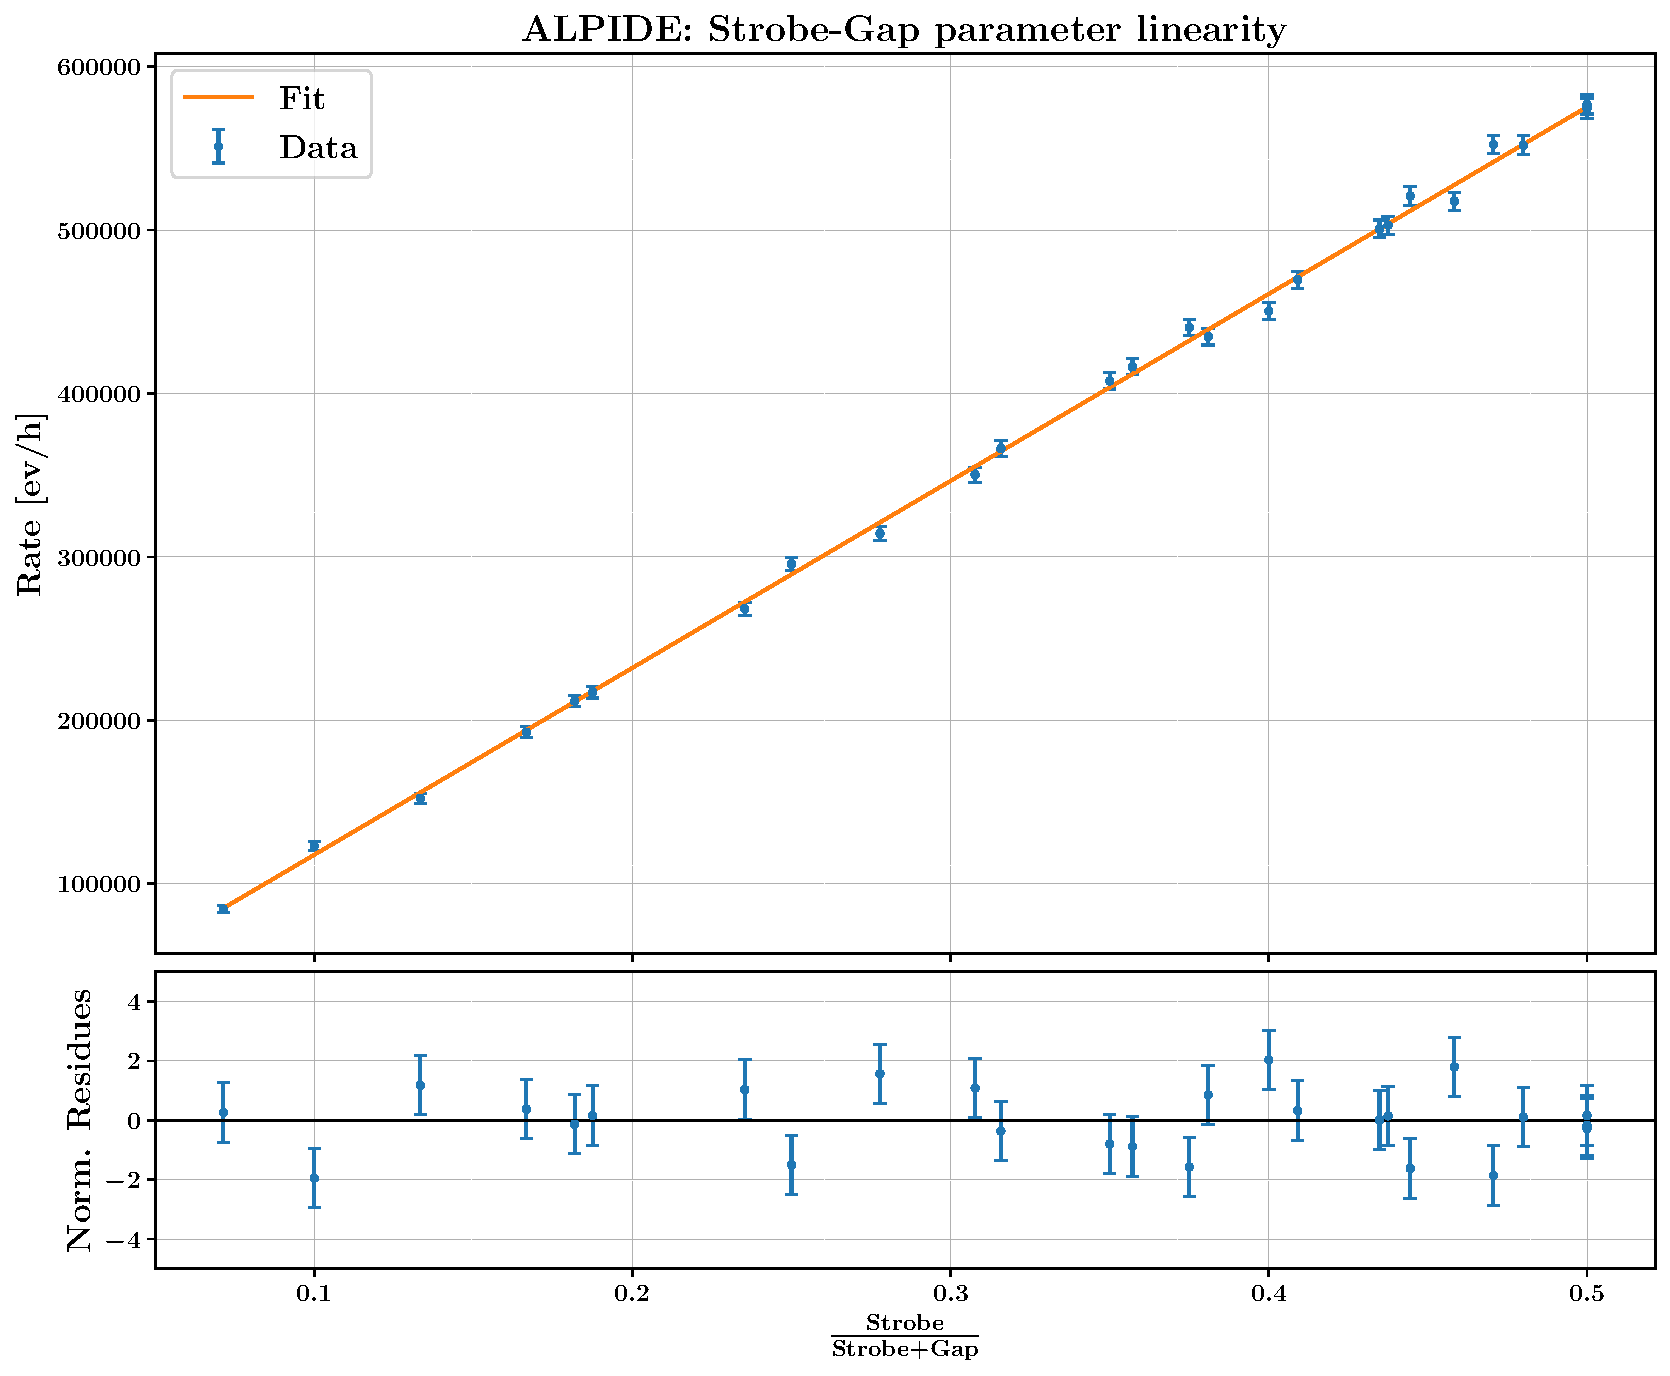
\includegraphics[width=1.0\linewidth, valign=c]{../sections/03/images/ALPIDE/ALPIDE_str_par.pdf}}
            \label{tab:strobe_data}
        }
    \end{minipage}
    \caption{Measurements of the acquired rate of events with different values of strobe and gap, which are given in units of clock cycles. In \figref{fig:strobe_plot}, the rate is plotted in function of the ratio of the strobe and strobe plus gap, namely \( r \), alongside with the linear fit performed and the normalised residuals. In \tabref{tab:strobe_data}, the acquired data and the results of the linear fit are reported.}
    \label{fig:strobe_analysis}
\end{figure*}

From the fit results, we observe how our data are compatible with a linear trend and so we can extrapolate useful information for the setup optimal working point:
\begin{itemize}
    \item the effective rate that we expect at zero angular position is the slope value $m$ of the linear fit;
    \item the intercept value $q$ is in good compatibility with the expected value of \( 0 \), which means that our measurements are not affected in a relevant way by systematic uncertainties;
    \item furthermore, both PCA ratio and cluster area do not show any dependence on the selected strobe-gap parameters.
\end{itemize}



\subsection{Radioactive source characterisation}

\paragraph{\( \alpha \) exit energy}
Focusing on the \( \alpha \) emissions of the source, we have previously listed the main decay product energies in \tabref{tab:source_emissions}. However, when detecting these particles, we will not find these exact energies. In fact, the active material of \( {}^{241}\mathrm{Am} \) is followed by multiple gold plates, which cause a partial loss of energy due to \textbf{straggling} effects. Dealing with this phenomenon is simple, but at the same time accurate, by following the same approach in \cite{alphaMC}. We model the energy loss with a Gaussian distribution \( f\qty(\mathcal{E}_{\mathrm{loss}})=G(\mu,\sigma) \), whose parameters are:
\begin{equation}
    \begin{aligned}
        \mu
        &=
            S(\mathcal{E}_\alpha)\rho\Delta x \\
        \sigma^{2}
        &=
            4 \pi
            \left(
                \frac{e^{2}}{4 \pi \varepsilon_{0}}
            \right)^{2}
            z_{\alpha}^{2} Z N \Delta x
    \end{aligned}
    \quad ,
\end{equation}
where:
\begin{itemize}
    \item \( S(\mathcal{E}_{\alpha}) \) is the material stopping power at \( \mathcal{E}_{\alpha} \) energy;
    \item \( z_{\alpha} \) and \( Z \) are the \( \alpha \) particle and the target atomic numbers, respectively;
    \item \( N \) is the number of atoms per unit of volume;
    \item \( \Delta x \) and \( \rho \) the gold plates total thickness (in \( \si{cm} \)) and density (in \( \si{g/cm^{3}} \)), respectively.
\end{itemize}
The beam distribution will be the convolution of three delta distributions (one for each decay channel), convolved with the corresponding energy loss distribution. Therefore, the spectrum of \( \alpha \) particles after traversing the gold plates can be modelled with the sum of three Gaussians\footnote{The convolution of a gaussian and a delta distribution can be computed as the convolution between two Gaussians, which is known to be a Gaussian distribution:
\begin{equation}
    G_1(\mu_1, \sigma_1) \circledast G_2(\mu_2, \sigma_2)
    =
    G\qty(\mu_1 +\mu_2, \sqrt{\sigma_1^2+\sigma_2^2})
    \Rightarrow
    G_1(\mu_1, \sigma_1) \circledast \delta(x-\mu_2)
    =
    G_1(\mu_1, \sigma_1) \circledast G_2(\mu_2, 0)
    =
    G(\mu_1 +\mu_2, \sigma_1)
\end{equation}}:
\begin{equation}
    f\qty(\mathcal{E}_{\mathrm{beam}})
    =
    \sum_{i} f_{i} G(\mathcal{E}_{i} - \mathcal{E}_{\mathrm{loss},i}, \sigma_i)
    \quad ,
\end{equation}
where \( f_{i} \) is the decay fraction of the \( i^{\mathrm{th}} \) channel and \( \mathcal{E}_{i} \), \( \mathcal{E}_{\mathrm{loss},i} \) and \( \sigma_{i} \) are the \( \alpha \) energy, energy loss and standard deviation in that specific channel, respectively. The contributions from all the relevant \( \alpha \) decay channels are showed in \figref{fig:preliminary_source_straggled_channels}, while the shape of the total estimated distribution is showed in \figref{fig:preliminary_source_straggled_total}. In particular, we find as peak energy:
\begin{equation}
    \mu_{\mathrm{peak}}
    =
    4.827 \ \si{MeV}
    \quad .
    \label{eq:preliminary_source_straggling_peak}
\end{equation}

\begin{figure*}[h]
    \centering
    \begin{minipage}[c]{0.49\linewidth}
        \vspace{0pt}
        \centering
        \subfloat[Straggled \( \alpha \) spectra for each decay channel]{
            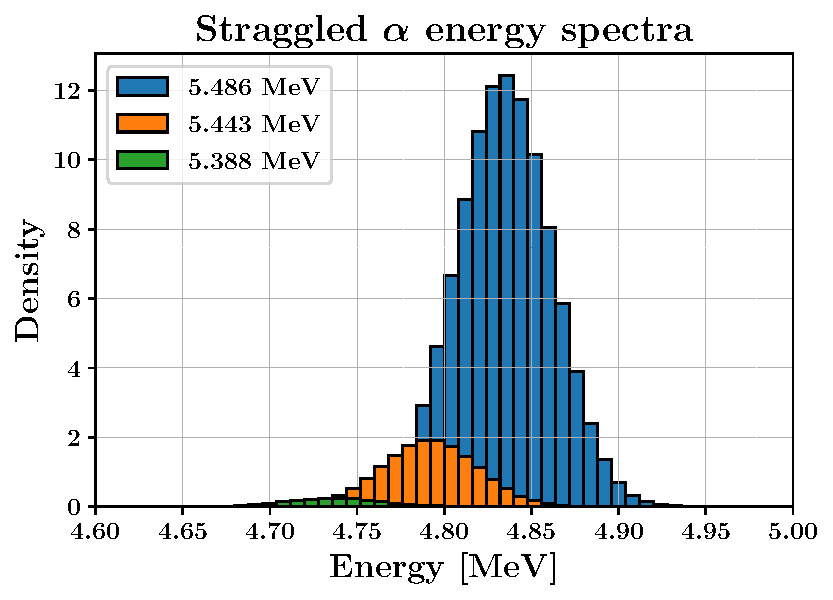
\includegraphics[height=6cm]{../sections/03/images/source/source_straggled_channels.pdf}
            \label{fig:preliminary_source_straggled_channels}
        }
    \end{minipage}%
    \hfill%
    \begin{minipage}[c]{0.49\linewidth}
        \vspace{0pt}
        \centering
        \subfloat[Straggled \( \alpha \) total spectrum]{
            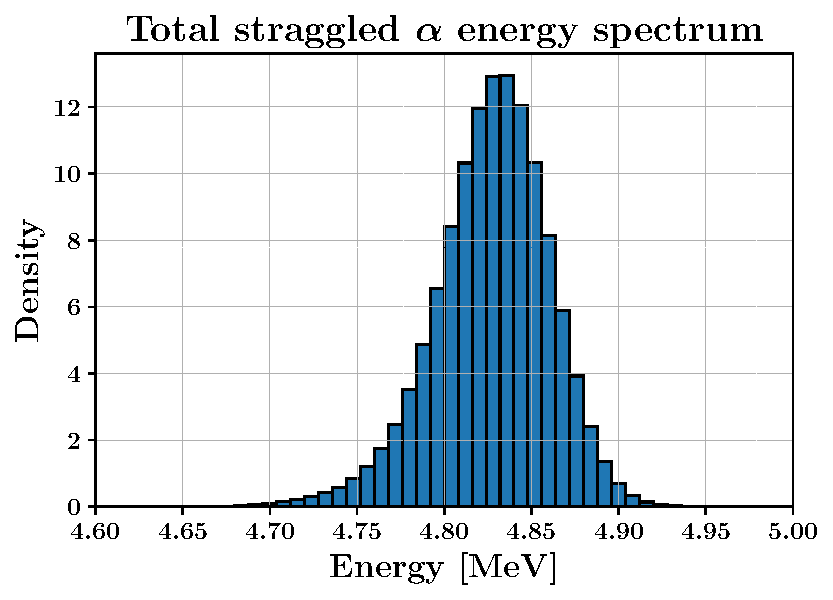
\includegraphics[height=6cm]{../sections/03/images/source/source_straggled_total.pdf}
            \label{fig:preliminary_source_straggled_total}
        }
    \end{minipage}%
    \caption{Estimated energy spectrum for the ${}^{241}\mathrm{Am}$ radioactive source after the passage from a gold plate of \( 1.51 \ \si{\mu m} \). In \textbf{\ref{fig:preliminary_source_straggled_channels}}, all the relevant contributions to the energy spectrum; in \textbf{\ref{fig:preliminary_source_straggled_total}}, the total energy spectrum density.}
    \label{fig:preliminary_source_straggled}
\end{figure*}


\paragraph{Source isotropy}
On the experimental side, after the calculations in the previous Paragraph on the energy loss of \( \alpha \) particles, we study the source isotropy of emission. This can be accomplished by placing the active material section of the source cylinder in the rotation axis of the support over the step motor. By this way, without collimating the beam, the SSB detector ``sees'' the source emissions also at large angles. Therefore, we can test if the rate of events is approximately the same in a certain angular range by fitting with \( y = w \). The results of this test are showed in \figref{fig:preliminary_source_isotropy}. As we can observe, the hypothesis of emission isotropy is reasonable, confirmed by the \( \chi^{2} \) over the degrees of freedom which is approximately \( 1 \).


\begin{figure*}[h]
    \begin{minipage}[c]{0.49\linewidth}
        \vspace{0pt}
        \centering
        \subfloat[Plot of measurements, fit and residuals]{
            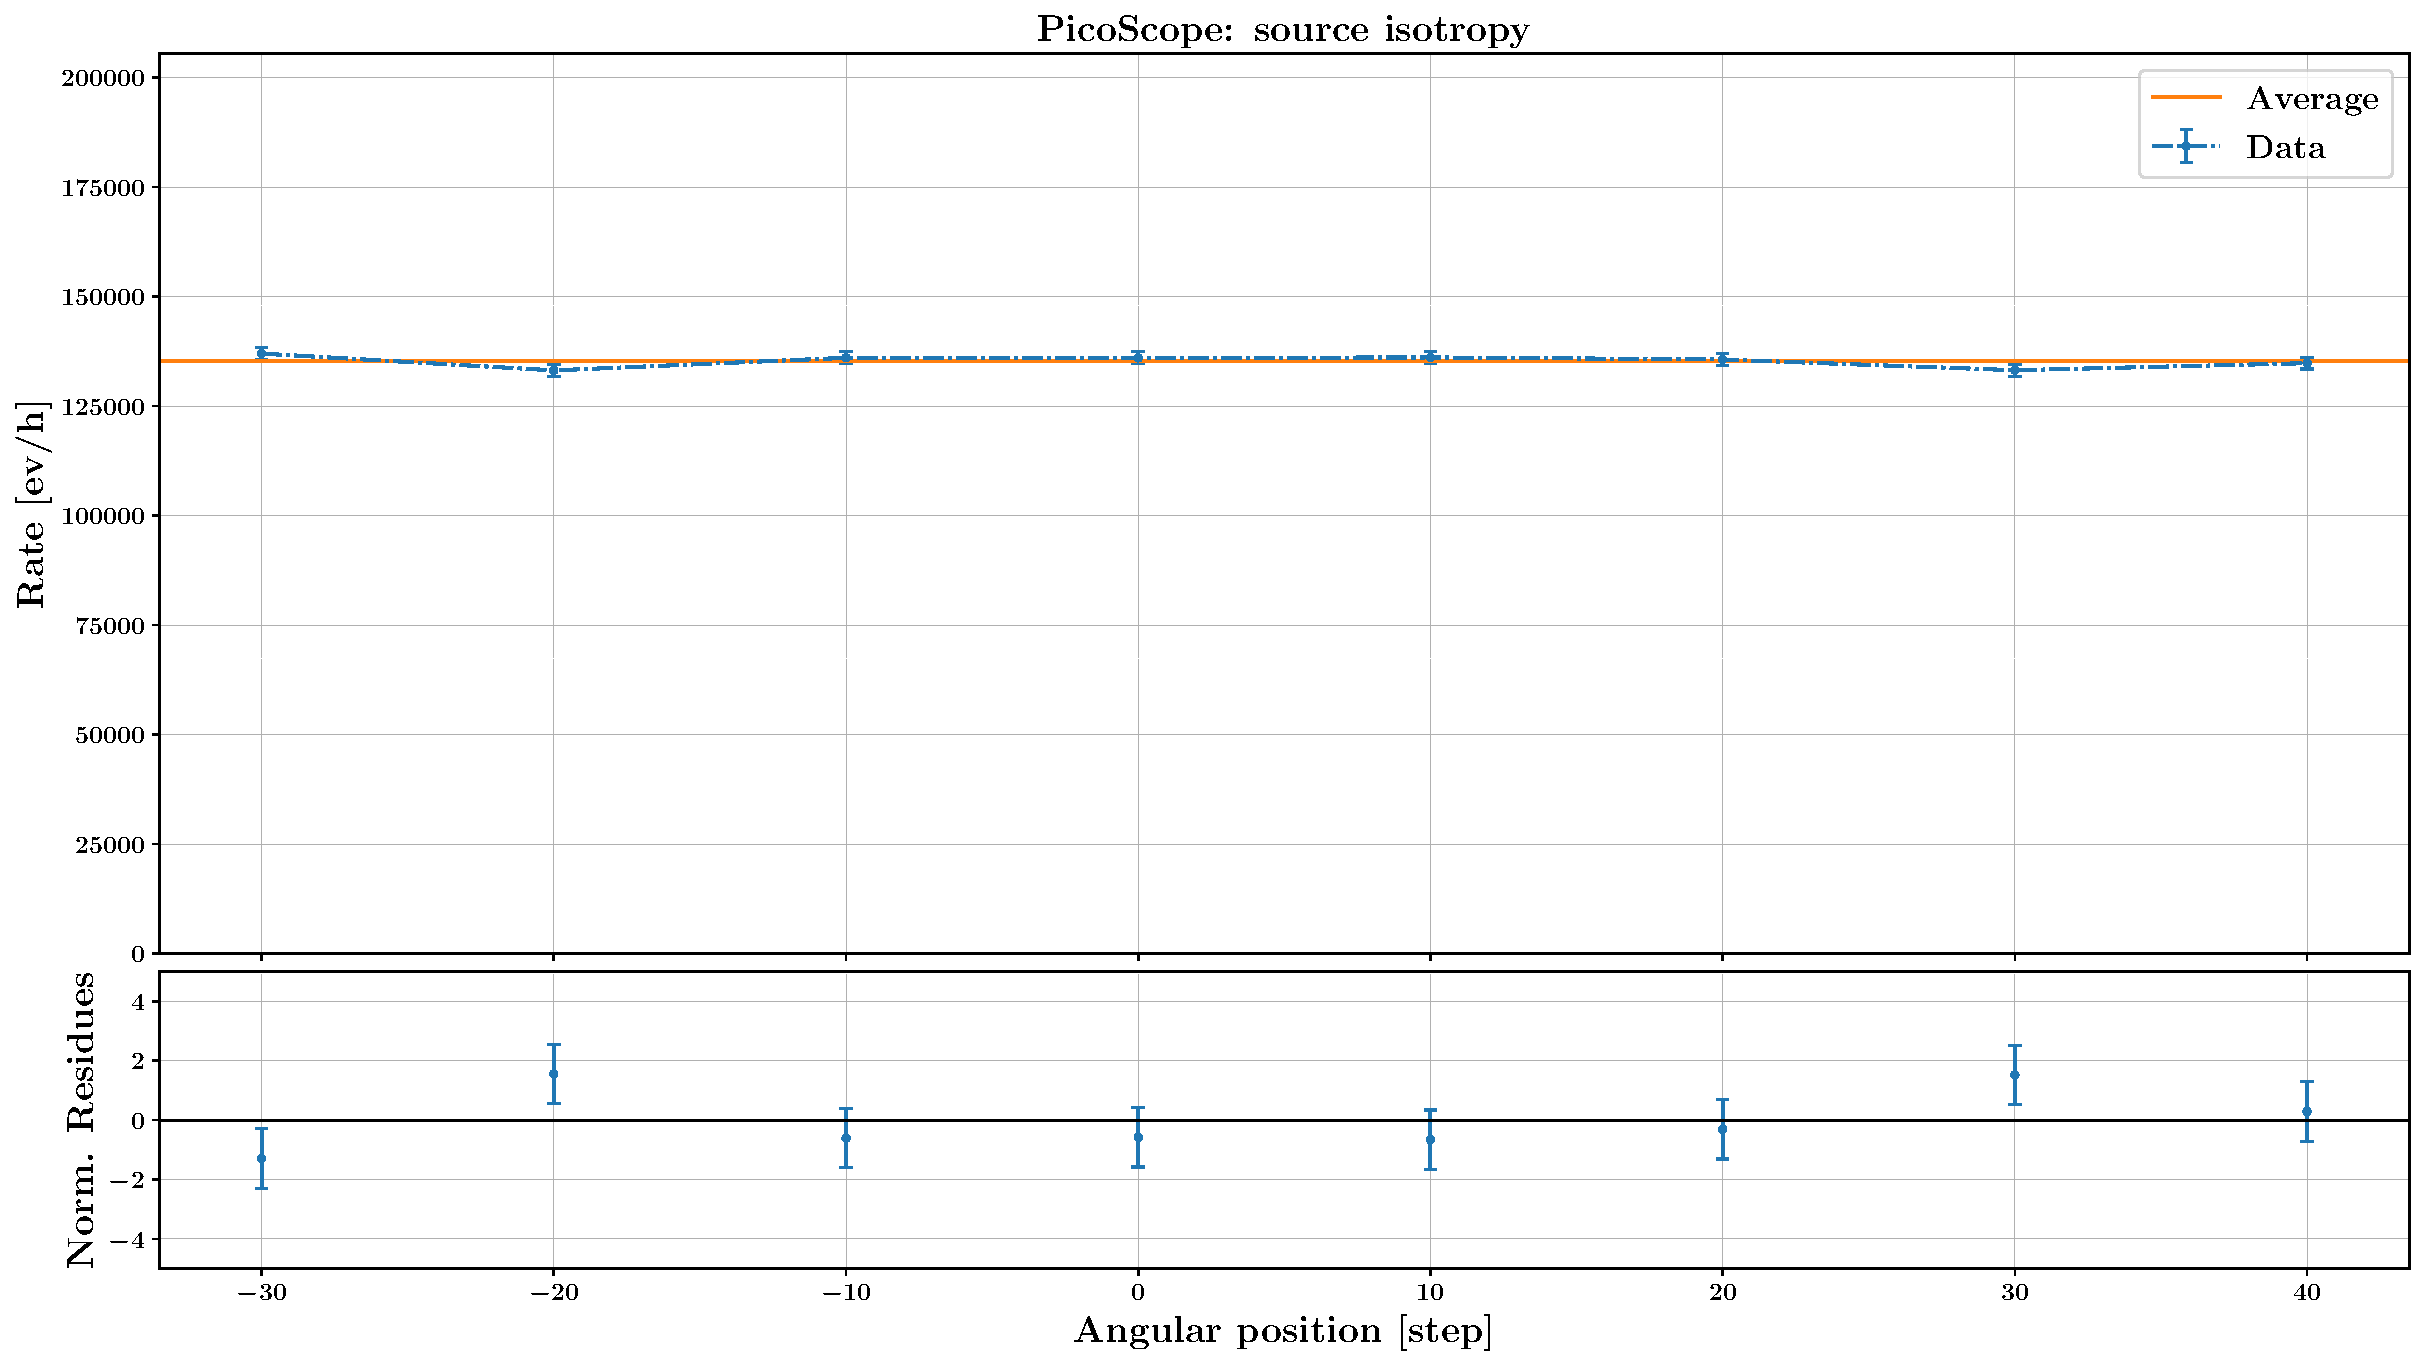
\includegraphics[width=1.0\linewidth, valign=c]{../sections/03/images/source/source_isotropy.pdf}
            \label{fig:preliminary_source_isotropy_plot}
        }
    \end{minipage}%
    \hfill%
    \begin{minipage}[c]{0.49\linewidth}
        \vspace{0pt}
        \centering
        \subfloat[Measurements and fit results]{
            \adjustbox{valign=c}{
            {\footnotesize
                \begin{tabular}{ccc}
                    \toprule
                    \multicolumn{3}{c}{\textbf{Data}}   \\
                    \colrule
                    \textbf{Angle [deg]}  &   \textbf{Exp. time [s]} &   \textbf{\boldmath Rate [\(10^{5} \cdot \) ev/h]} \\
                    \colrule
                    \( -36.0 \) &   \( 268.5 \)   & \( 1.346 \pm 0.001 \) \\
                    \( -27.0 \) &   \( 262.8 \)   & \( 1.370 \pm 0.001 \) \\
                    \( -18.0 \) &   \( 270.4 \)   & \( 1.331 \pm 0.001 \) \\
                    \( - 9.0 \) &   \( 264.6 \)   & \( 1.360 \pm 0.001 \) \\
                    \(   0.0 \) &   \( 264.7 \)   & \( 1.360 \pm 0.001 \) \\
                    \(   9.0 \) &   \( 264.5 \)   & \( 1.361 \pm 0.001 \) \\
                    \(  18.0 \) &   \( 265.4 \)   & \( 1.356 \pm 0.001 \) \\
                    \(  27.0 \) &   \( 270.3 \)   & \( 1.332 \pm 0.001 \) \\
                    \(  36.0 \) &   \( 267.0 \)   & \( 1.348 \pm 0.001 \) \\
                    \colrule
                    \multicolumn{3}{c}{\textbf{Fit results}}   \\
                    \colrule
                    {\boldmath\textbf{\( w \ \mathrm{[10^{5} \cdot ev/h]} \)}}  &   \multicolumn{2}{c}{\( 1.3514 \pm 0.0005 \)}   \\
                    {\boldmath\( \chi^{2} \)}  &   \multicolumn{2}{c}{\( 7.94 \)}   \\
                    {\boldmath\( \mathrm{d.o.f.} \)}  &   \multicolumn{2}{c}{\( 8 \)}   \\
                    \botrule
                \end{tabular}
            }
            }
            \vphantom{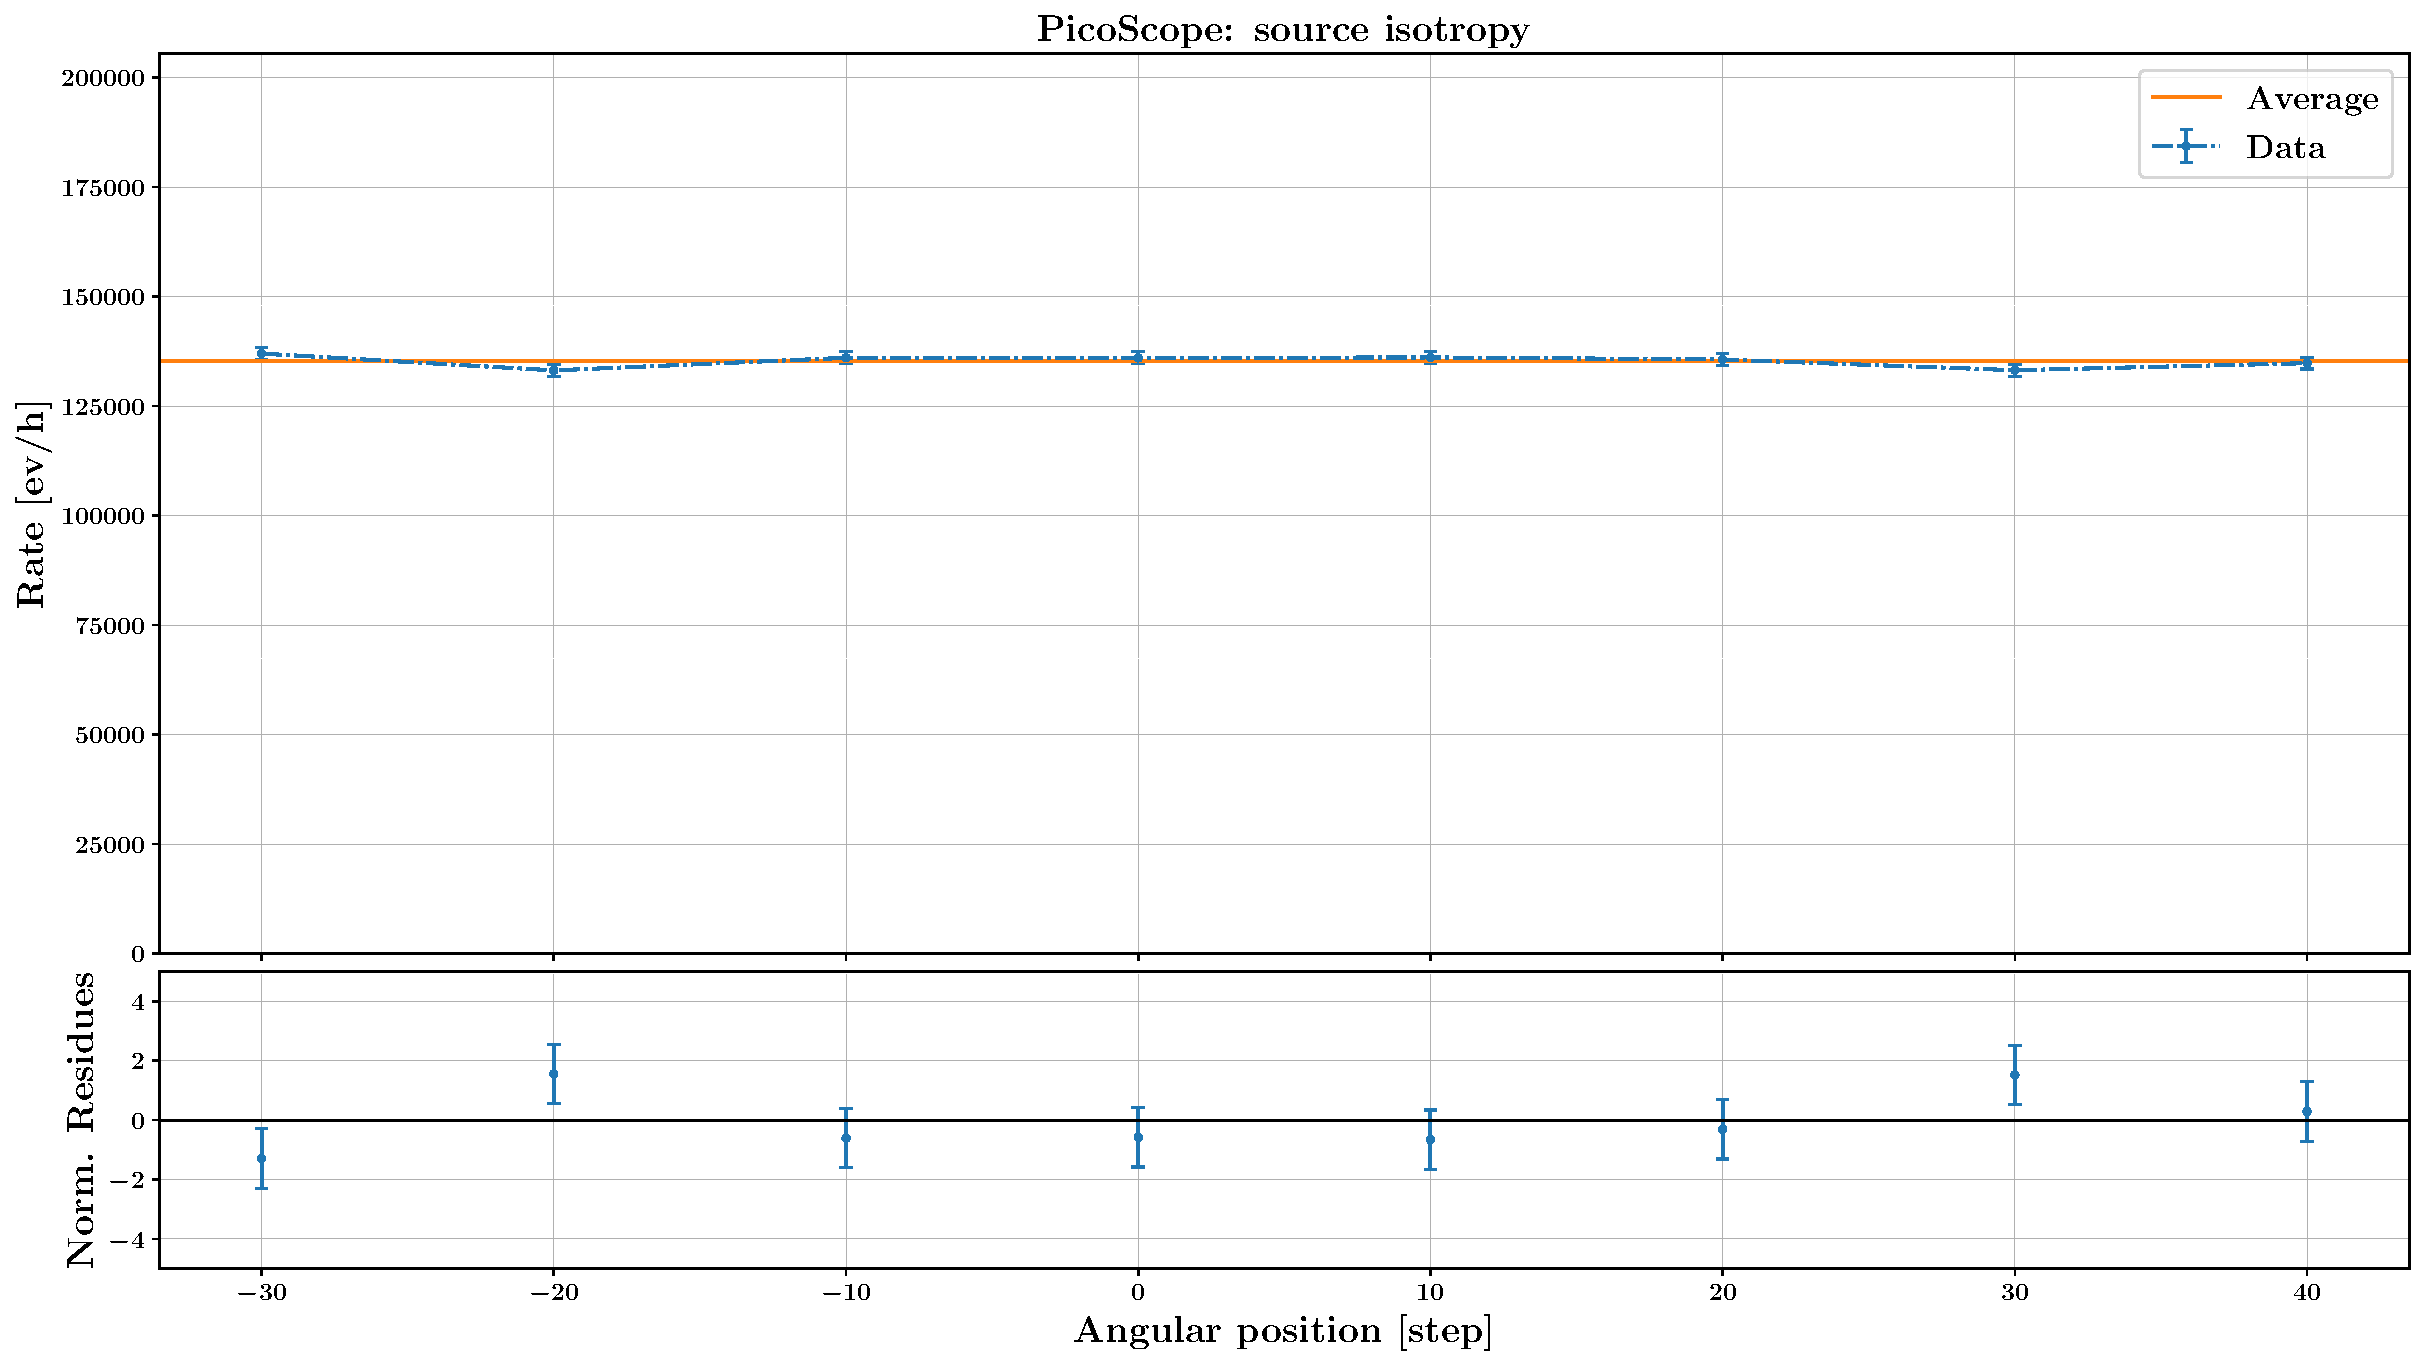
\includegraphics[width=1.0\linewidth, valign=c]{../sections/03/images/source/source_isotropy.pdf}}
            \label{tab:preliminary_source_isotropy_data}
        }
    \end{minipage}
    \caption{Measurements with emission point approximately in the axis of rotation and at different angular positions. In \textbf{\ref{fig:preliminary_source_isotropy_plot}}, the average weighted on the inverse squared of errors is reported as a straight line and the related residues are showed in the bottom panel. In \textbf{\ref{tab:preliminary_source_isotropy_data}}, we report all the experimental measurements obtained to reproduce the plot, along with the fit results.}
    \label{fig:preliminary_source_isotropy}
\end{figure*}


\paragraph{Source emissions energy-angle correlation}
The last study of source characterisation concerns the \( \alpha \) particle energy correlation with the angular direction of emission. Let us consider the same configuration employed in the previous Paragraph, so the source point of emission in the centre of rotation of the motor. In principle, an \( \alpha \) particle emitted at a larger angle with respect to zero is affected by larger straggling effects, since it goes through a longer thickness of gold plate. So, we expect to observe a spectrum peak energy lower for greater angles and higher for angles near to the zero.

Before performing this study on the same dataset employed for the study of source isotropy, we define an energy calibration strategy for the energy spectrum. In the previous discussion, it has been expressed in arbitrary units. However, now that we know the central angle energy spectrum and so its peak in \( \si{MeV} \) from previous calculations, we can use this information to solve this problem. In fact:
\begin{itemize}
    \item we set as zero of the energy in \( \si{MeV} \) the zero of the energy in arbitrary units;
    \item we set the peak energy in arbitrary units for the spectrum at zero position to the value in \eqnref{eq:preliminary_source_straggling_peak}. 
\end{itemize}
By this way, we can extrapolate a calibration line from the data acquired at zero angular position and use it to calibrate the energy spectra for the other positions. The next operation is to take the peak energy in \( \si{MeV} \) for each case and check if it decreases for wider angles. The results for this study are showed in \figref{fig:preliminary_source_angle_energy_correlation}, where we model the trend of data by fitting with the following function:
\begin{equation}
    y(\theta)
    =
    a + \frac{b}{\cos\qty(\theta-c)}
    \quad ,
    \label{eq:preliminary_source_angle_energy_correlation_fit}
\end{equation}
which represents the theoretical expectation due to geometrical and trigonometric considerations.

Now, of we consider the working point of a collimated beam, namely a beam concentrated in the angular region \( [-10,10] \) degrees, we observe that the energy variation in function of the angle is a secondary effect. In fact, we would have an energy variation of about one hundred of keVs around the maximum peak energy in \eqnref{eq:preliminary_source_straggling_peak}.


\begin{figure*}[h]
    \begin{minipage}[c]{0.49\linewidth}
        \vspace{0pt}
        \centering
        \subfloat[Plot of measurements, fit and residuals]{
            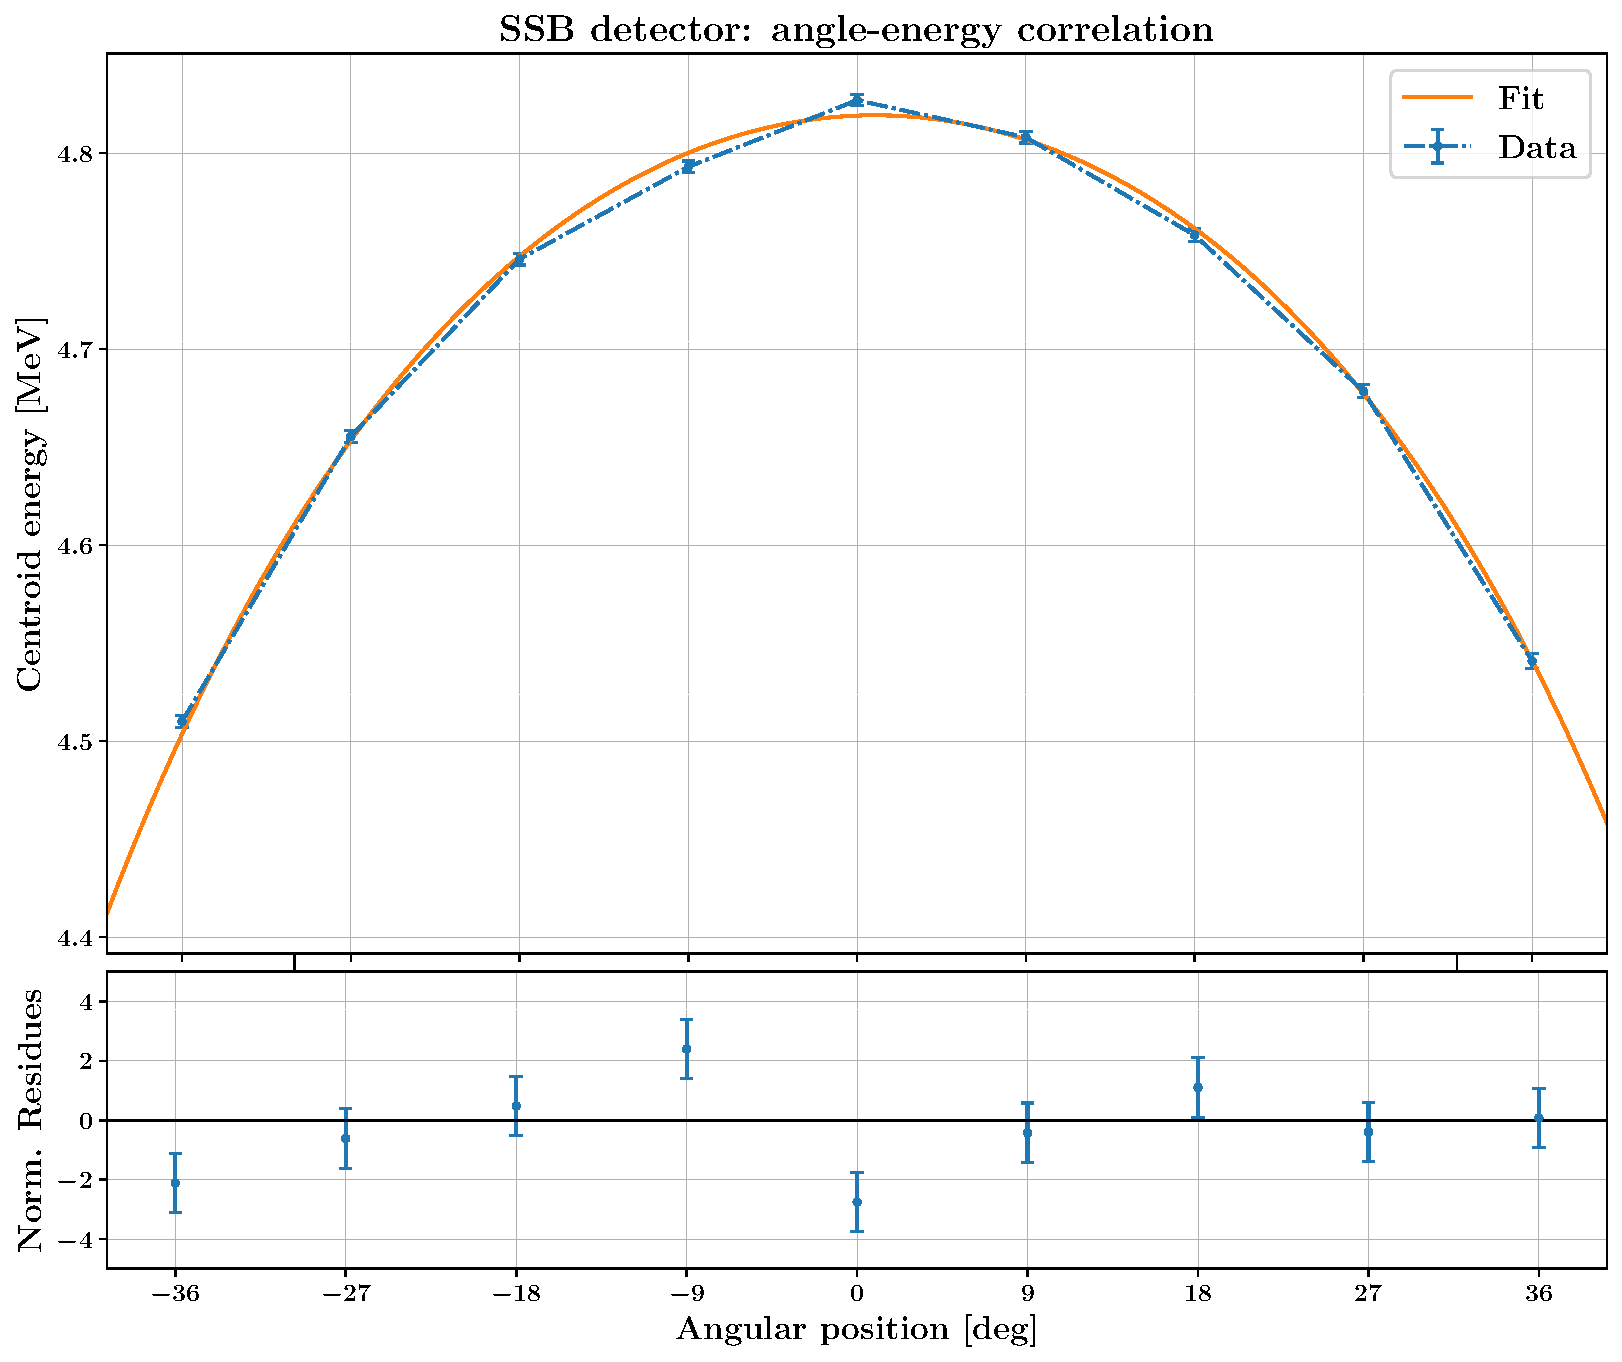
\includegraphics[width=1.0\linewidth, valign=c]{../sections/03/images/source/source_correlation.pdf}
            \label{fig:preliminary_source_angle_energy_correlation_plot}
        }
    \end{minipage}%
    \hfill%
    \begin{minipage}[c]{0.49\linewidth}
        \vspace{0pt}
        \centering
        \subfloat[Measurements and fit results]{
            \adjustbox{valign=c}{
            {\footnotesize
                \begin{tabular}{ccc}
                    \toprule
                    \multicolumn{3}{c}{\textbf{Data}}   \\
                    \colrule
                    \textbf{Angle [deg]}  &   \textbf{Exp. time [s]} &   \textbf{\boldmath\( \mu(\theta) \) [MeV]} \\
                    \colrule
                    \( -36.0 \) &   \( 268.5 \)   & \( 4.510 \pm 0.003 \) \\
                    \( -27.0 \) &   \( 262.8 \)   & \( 4.655 \pm 0.003 \) \\
                    \( -18.0 \) &   \( 270.4 \)   & \( 4.746 \pm 0.003 \) \\
                    \( - 9.0 \) &   \( 264.6 \)   & \( 4.793 \pm 0.003 \) \\
                    \(   0.0 \) &   \( 264.7 \)   & \( 4.827 \pm 0.003 \) \\
                    \(   9.0 \) &   \( 264.5 \)   & \( 4.808 \pm 0.003 \) \\
                    \(  18.0 \) &   \( 265.4 \)   & \( 4.758 \pm 0.003 \) \\
                    \(  27.0 \) &   \( 270.3 \)   & \( 4.679 \pm 0.003 \) \\
                    \(  36.0 \) &   \( 267.0 \)   & \( 4.541 \pm 0.004 \) \\
                    \colrule
                    \multicolumn{3}{c}{\textbf{Fit results}}   \\
                    \colrule
                    {\boldmath\textbf{\( a \ \mathrm{[MeV]} \)}}  &   \multicolumn{2}{c}{\( 6.08 \pm 0.03 \)}   \\
                    {\boldmath\textbf{\( b \ \mathrm{[MeV]} \)}}  &   \multicolumn{2}{c}{\(-1.26 \pm 0.03 \)}   \\
                    {\boldmath\textbf{\( c \ \mathrm{[rad]} \)}}  &   \multicolumn{2}{c}{\( 0.017 \pm 0.004 \)}   \\
                    {\boldmath\( \chi^{2} \)}  &   \multicolumn{2}{c}{\( 20.0 \)}   \\
                    {\boldmath\( \mathrm{d.o.f.} \)}  &   \multicolumn{2}{c}{\( 6 \)}   \\
                    \botrule
                \end{tabular}
            }
            }
            \vphantom{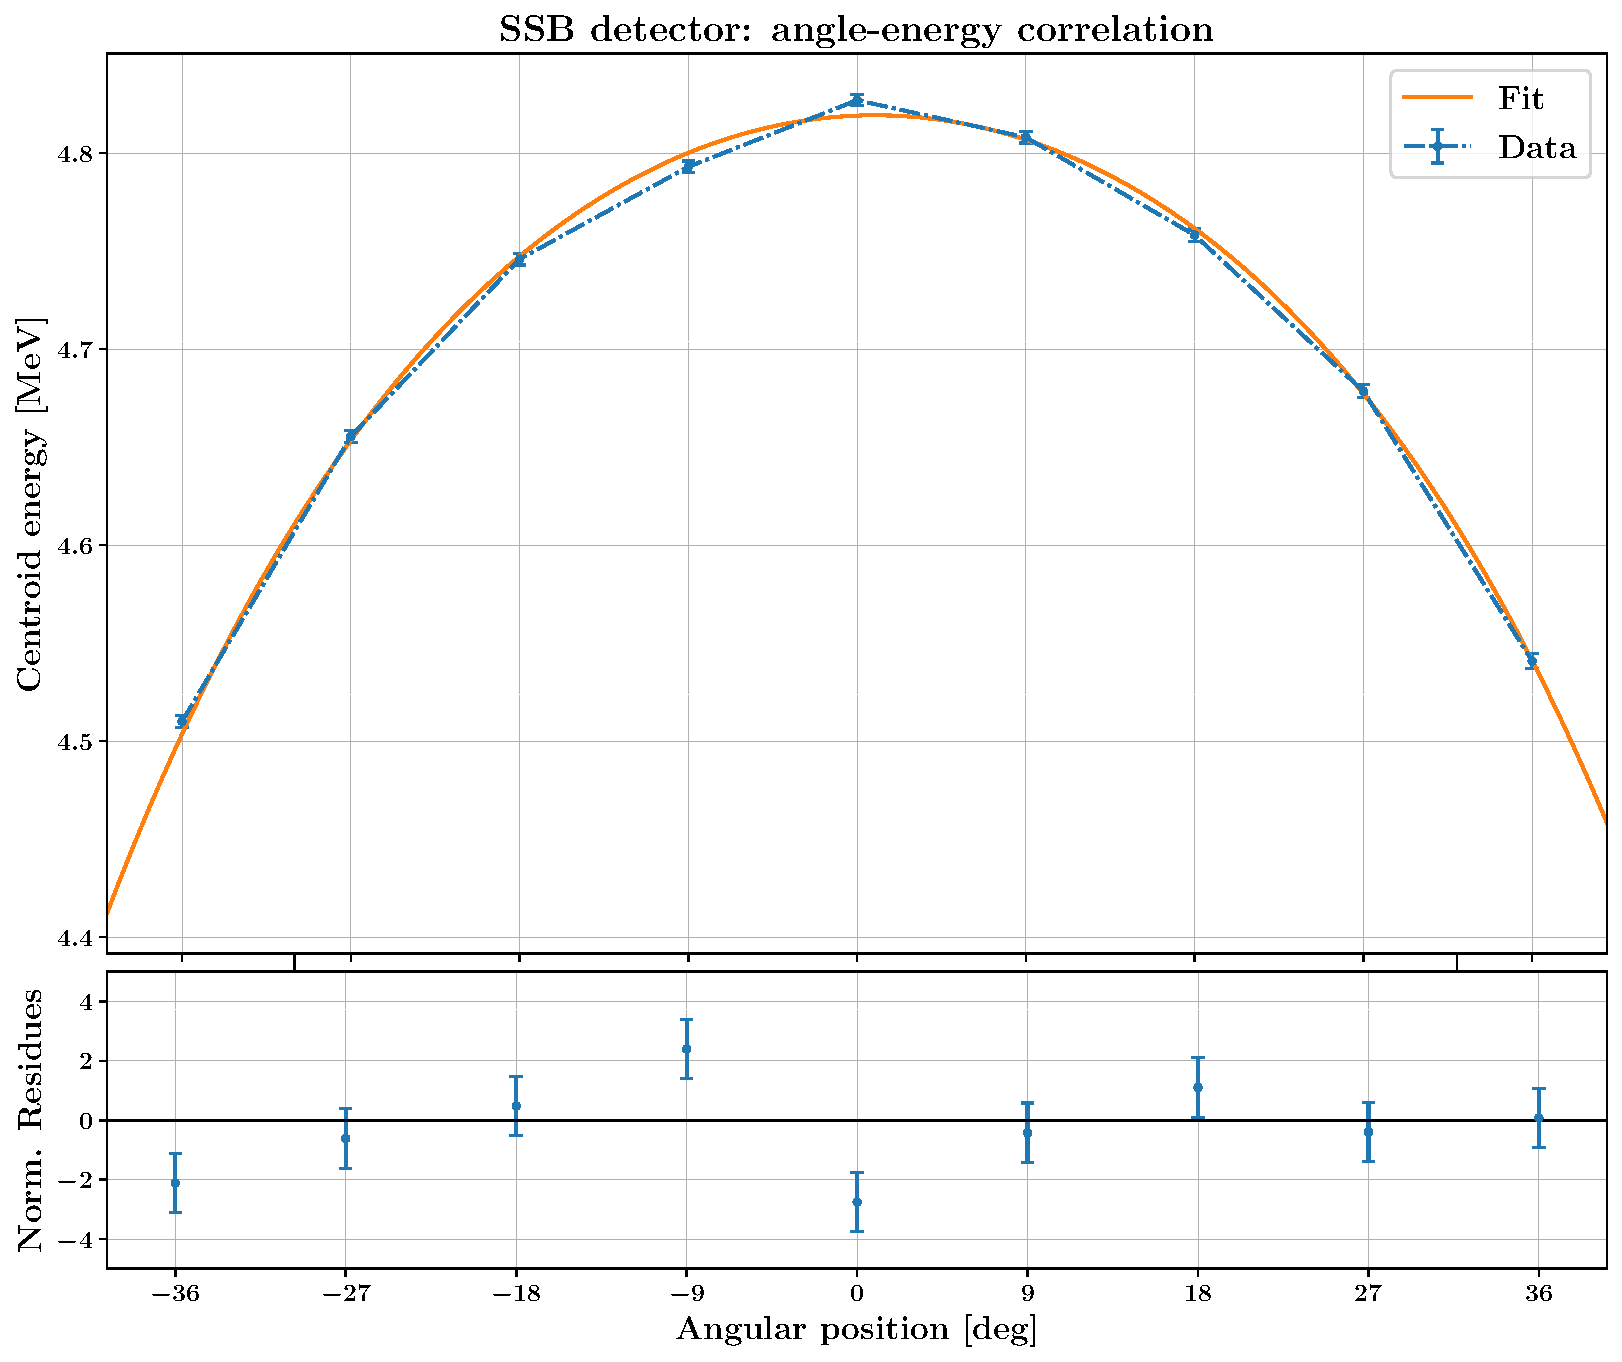
\includegraphics[width=1.0\linewidth, valign=c]{../sections/03/images/source/source_correlation.pdf}}
            \label{tab:preliminary_source_angle_energy_correlation_data}
        }
    \end{minipage}
    \caption{Measurements with emission point approximately in the axis of rotation and at different angular positions. In \textbf{\ref{fig:preliminary_source_angle_energy_correlation_plot}}, the centroid energy in function of the angular position is plotted and fitted with \eqnref{eq:preliminary_source_angle_energy_correlation_fit}, with the residuals in the bottom panel. In \textbf{\ref{tab:preliminary_source_angle_energy_correlation_data}}, we report all the experimental measurements obtained to reproduce the plot, along with the fit results.}
    \label{fig:preliminary_source_angle_energy_correlation}
\end{figure*}



















\subsection{Simulation of the apparatus}

After having discussed all the needed characterisations of the apparatus components, we pass to the simulation of the experiment in order to model the behaviour of the apparatus itself. In particular, we simulate both the conditions of scattering foil removed or inserted, so that we can obtain a model of both the beam and scattering profiles. Moreover, we can repeat this simulation for a different foil material by simply changing its intrinsic parameters, such as its atomic number and density.

Before going on, we remark that the physics of scattering is based on the differential cross section expression in \eqnref{eq:S01_1}. In addition, we improve the model by introducing geometrical, trigonometric and physical factors, such as beam angular spread, the dimensions of the collimators of the beam and of the detectors, and the source products energy spread. The last remark to do is that the  system of reference chosen has its origin in the centre of the vacuum chamber, the \( z \)-axis parallel to the beam direction and the \( y \)-axis pointing upward perpendicularly to the vacuum chamber surface. In order to fit the simulation to our setup, the positions of all the setup components are set to the values listed in the previous sections.


\paragraph{Particle generation}
Given the source surface centre \( x_{\mathrm{s},0} \) and its radius \( r_{\mathrm{s}} = 0.335 \ \si{mm} \), a specified number of particles is generated with energy \( \mathcal{E}_{\alpha} \) taken from the distribution in \figref{fig:preliminary_source_straggled_total}. Then, each particle is associated to a position $(x_{i},y_{i},z_{i})$, uniformly generated inside the source surface, and to a momentum, randomly generated in the forward hemisphere with kinematics coherent with the sampled energy.


\paragraph{Beam collimation}
After the generation on the source surface, the kinematic evolution of each particle is analytically computed up to the plane of the first beam collimator. Denoting by $w$ and $h$ the height and width,  respectively, of the collimator, the following conditions are imposed in order to further evolve the path of a particle:
\begin{equation}
    \begin{cases}
        \abs{x_{i} - x_{\mathrm{C1}}} \leq \frac{w}{2}  \\
        \abs{y_{i} - y_{\mathrm{C1}}} \leq \frac{h}{2}
    \end{cases}
    \quad ,
\end{equation}
where \( x_{\mathrm{C1}} \) and \( y_{\mathrm{C1}} \) are the abscissa and the ordinate of the first collimator, respectively. The particles not satisfying both the conditions are discarded and the same procedure is applied again after the spatial evolution to the plane of the second collimator. The particles exiting from the ladder are kept.


\paragraph{Target scattering}
The interaction with the gold foil is composed of the following passages:
\begin{itemize}
    \item for each particle an impact parameter \( b \) is randomly generated between \( 0 \) and the mean inter-atomic distance between the atoms;
    \item then, the scattering angle is computed in the intrinsic frame of the particle. With respect to this frame, the azimuth angle \( \alpha \) is randomly generated in \( [0,2\pi] \), while the polar angle is computed from the impact parameter as:
    \begin{equation}
        \theta
        =
        \pi - 2\cos^{-1} \qty[\frac{
            \displaystyle
            \frac{k}{2\mathcal{E}_{\alpha} b}
        }{
            \displaystyle
            \sqrt{
                1 + \qty( \frac{k}{2 \mathcal{E}_{\alpha} b} )^{2}
            }
        }]
        \qquad \text{with} \quad
        k
        =
        \frac{q_{\alpha} Z}{4 \pi \varepsilon_{0}}
        \quad ,
    \end{equation}
    where \( q_{\alpha} \) is the charge of the \( \alpha \) particle and \( Z \) the atomic number of the target.
    \item each particle momentum is rotated from the intrinsic frame to the laboratory frame by an opportune combination of rotation matrices, obtained from the scattering angles.
\end{itemize}

In the implementation of the computations described earlier, the following corrections are also included in order to improve the accuracy of simulation of the intrinsic physics:
\begin{itemize}
    \item atomic charge screening: the effective charge seen by the particle is not equal to \( Ze \), but it depends on the impact parameter. This effect is modelled by a (descending) exponential distribution, whose maximum is equal to \( Z \) for \( b = 0 \ \si{nm} \) and it saturates at a characteristic value \( Z' \) at the atomic radius \( r_{\mathrm{a}} \);
    \item energy loss due to straggling with foil: each particle energy and momentum is reduced according to the energy loss of a charge carrier when traversing a foil of a certain material.
\end{itemize}


\paragraph{Detector acquisition}
Similarly to what has been already done for the collimators, the detection of the scattered particles is implemented by spatially evolve them up to a distance from the centre of rotation of the motor equal to distance from the detectors, given in \tabref{tab:mechanics_support_distances}. In particular, for the specific case of SSB and ALPIDE detectors, the particles are respectively required to satisfy:
\begin{equation}
    \begin{aligned}
        \abs{y_{i} - y_{\mathrm{CD}}} &\leq \frac{r_{\mathrm{p}}}{2} \\
        \abs{y_{i} - y_{\mathrm{CD}}} &\leq \frac{h}{2}
    \end{aligned}
    \quad ,
\end{equation}
with \( r_{p} \) being the radius of the collimator of SSB detector and \( h \) the height of ALPIDE detector matrix. Lastly, the particles that are not discarded are the ones detected. Thus, from their final position it is possible to extract their angular position and, then, to compute the final angular distribution, taking as reference the centre of rotation of the motor and of the vacuum chamber.



\subsection{Characterisation of beam profile and validation of simulation}
In order to validate the simulation implementation and its results, we take as benchmark the beam profile of the radioactive source, namely the final angular distribution measured without the scattering foil. On the simulation side, we replicate this setup by not inserting the scattering foil in the apparatus simulated components. The comparison between the simulated and the experimental angular distributions of the beam is showed in \figref{fig:profile_picoscope} and \figref{fig:profile_ALPIDE}, respectively for SSB and ALPIDE detectors. It is possible to observe how the simulation replicates the trend of the experimental angular distribution, validating the implementation of the model.

\begin{figure*}[h]
    \begin{minipage}[c]{0.49\linewidth}
        \vspace{0pt}
        \centering
        \subfloat[SSB detector beam profile]{
            % 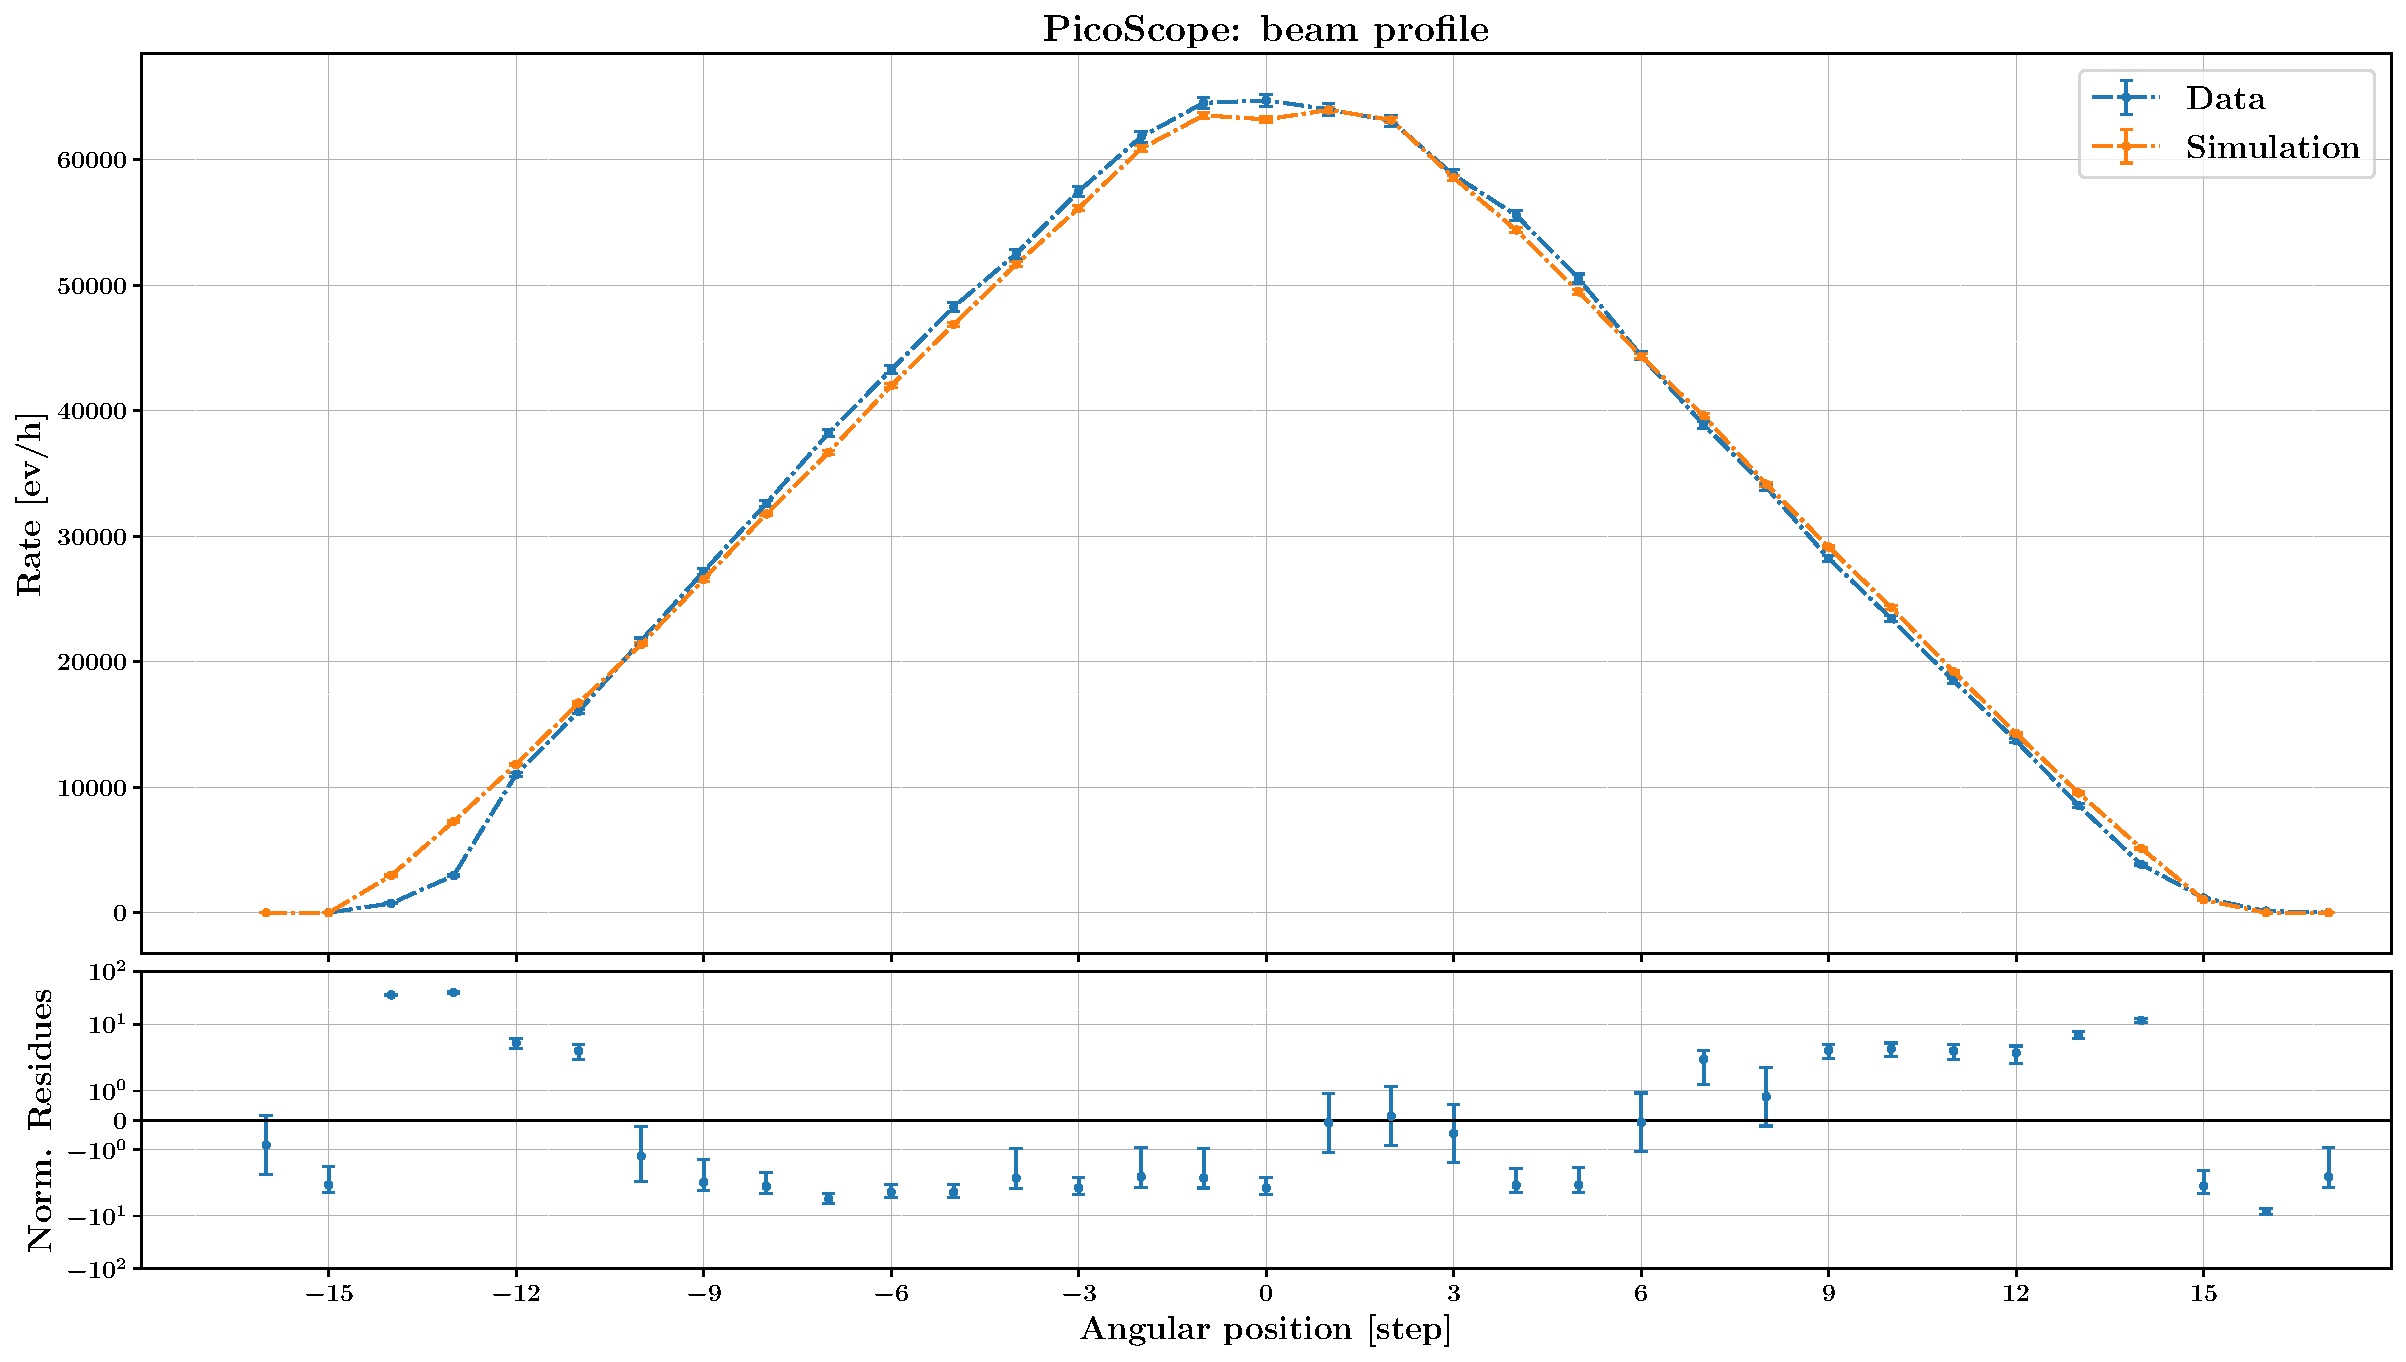
\includegraphics[width=\textwidth]{../sections/04/images/picoscope/beam_profile.pdf}
            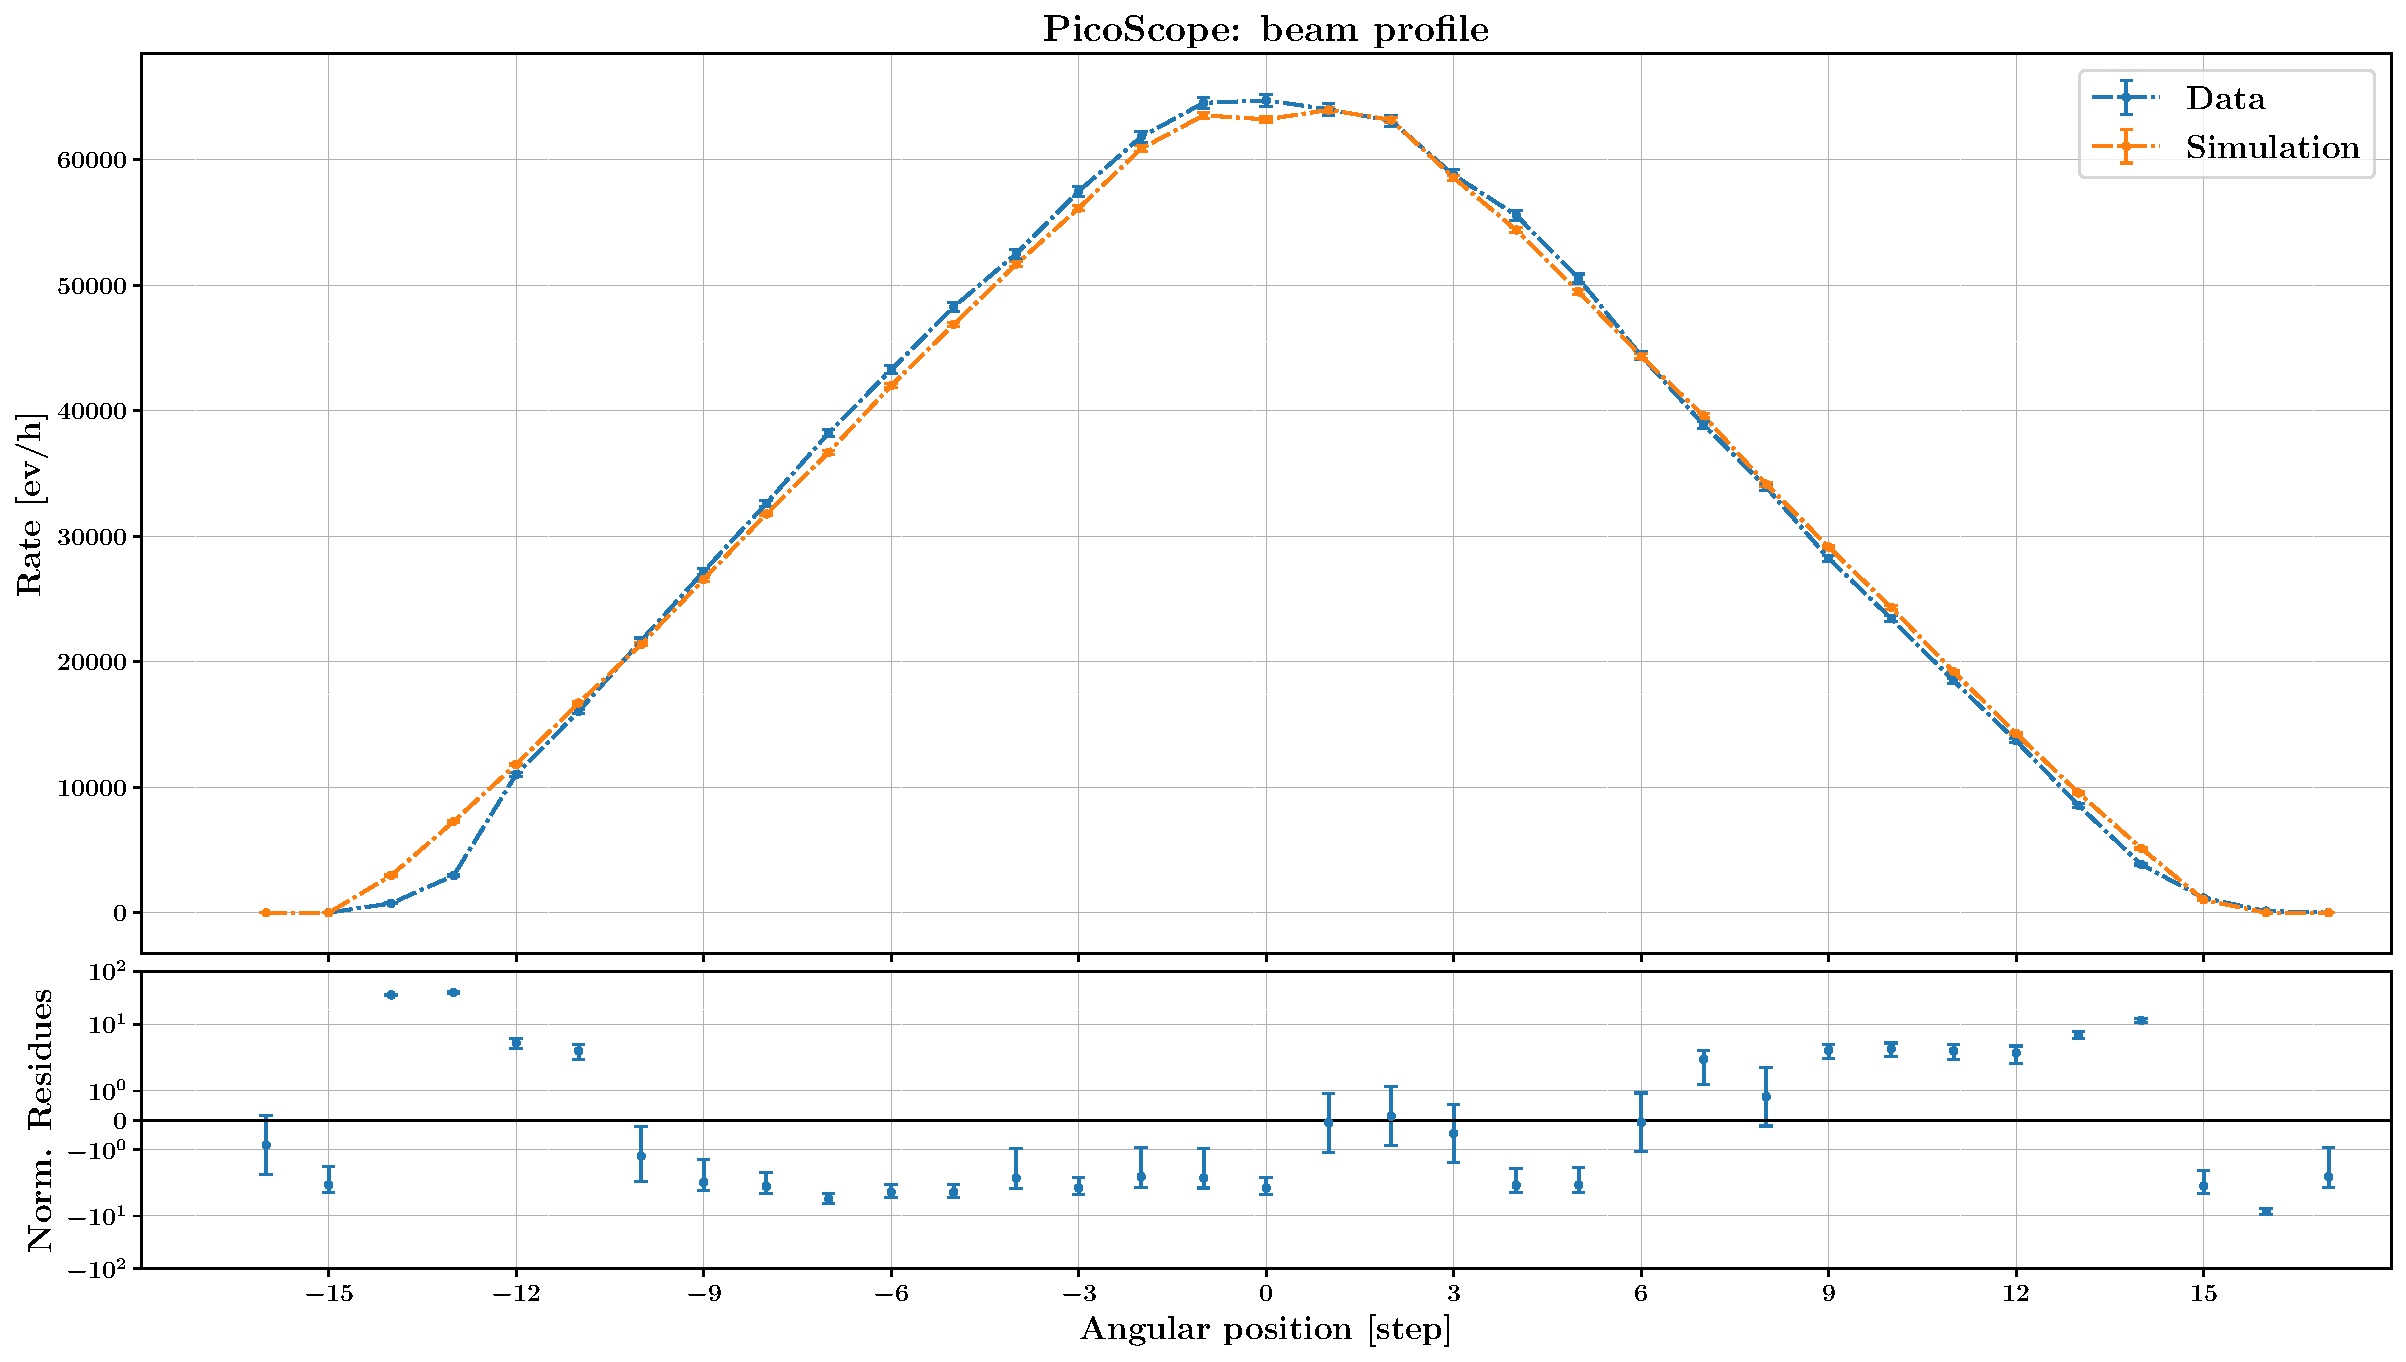
\includegraphics[height=6.5cm]{../sections/04/images/picoscope/beam_profile.pdf}
            \label{fig:profile_picoscope}
        }
    \end{minipage}
    \hfill
    \begin{minipage}[c]{0.49\linewidth}
        \vspace{0pt}
        \centering
        \subfloat[ALPIDE detector beam profile]{
            % 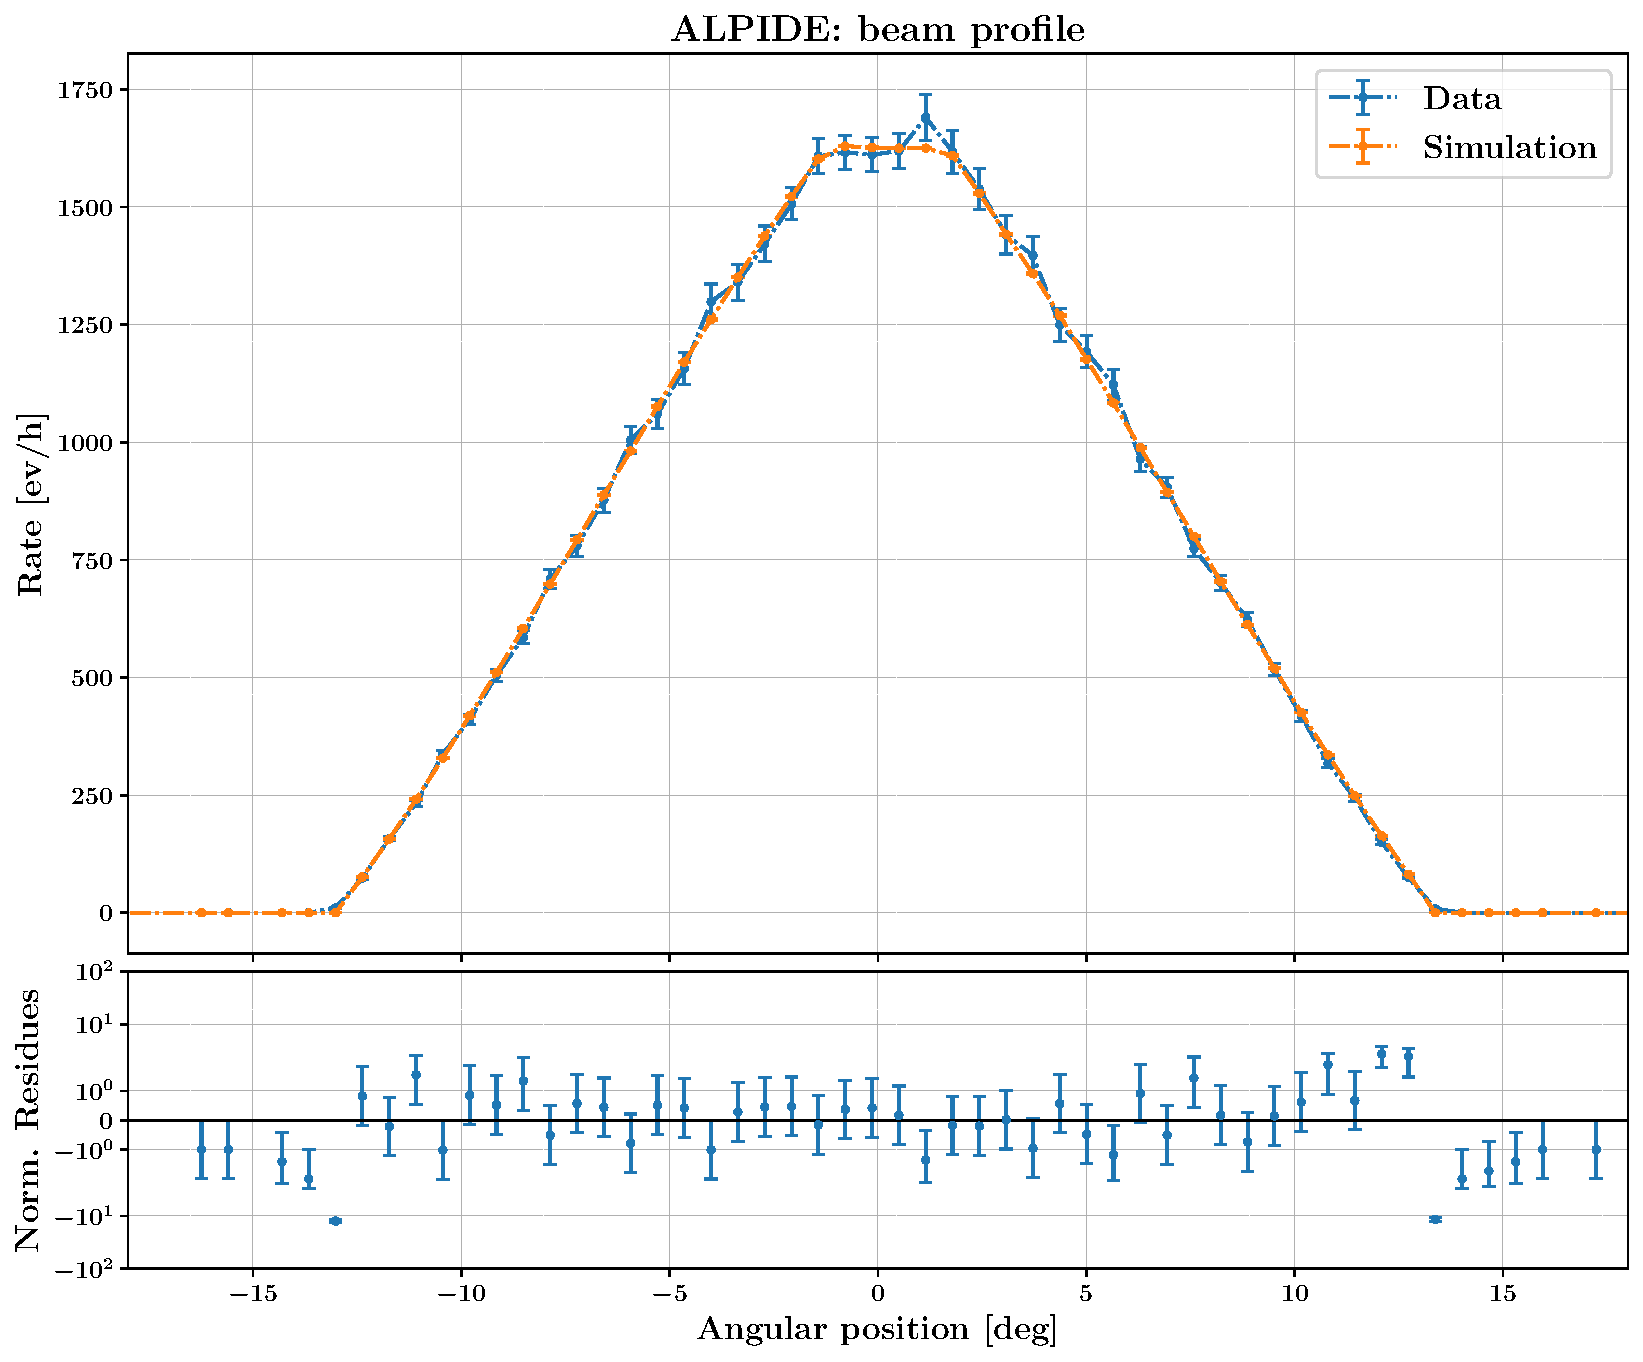
\includegraphics[width=\textwidth]{../sections/04/images/ALPIDE/ALPIDE_beam_profile.pdf}
            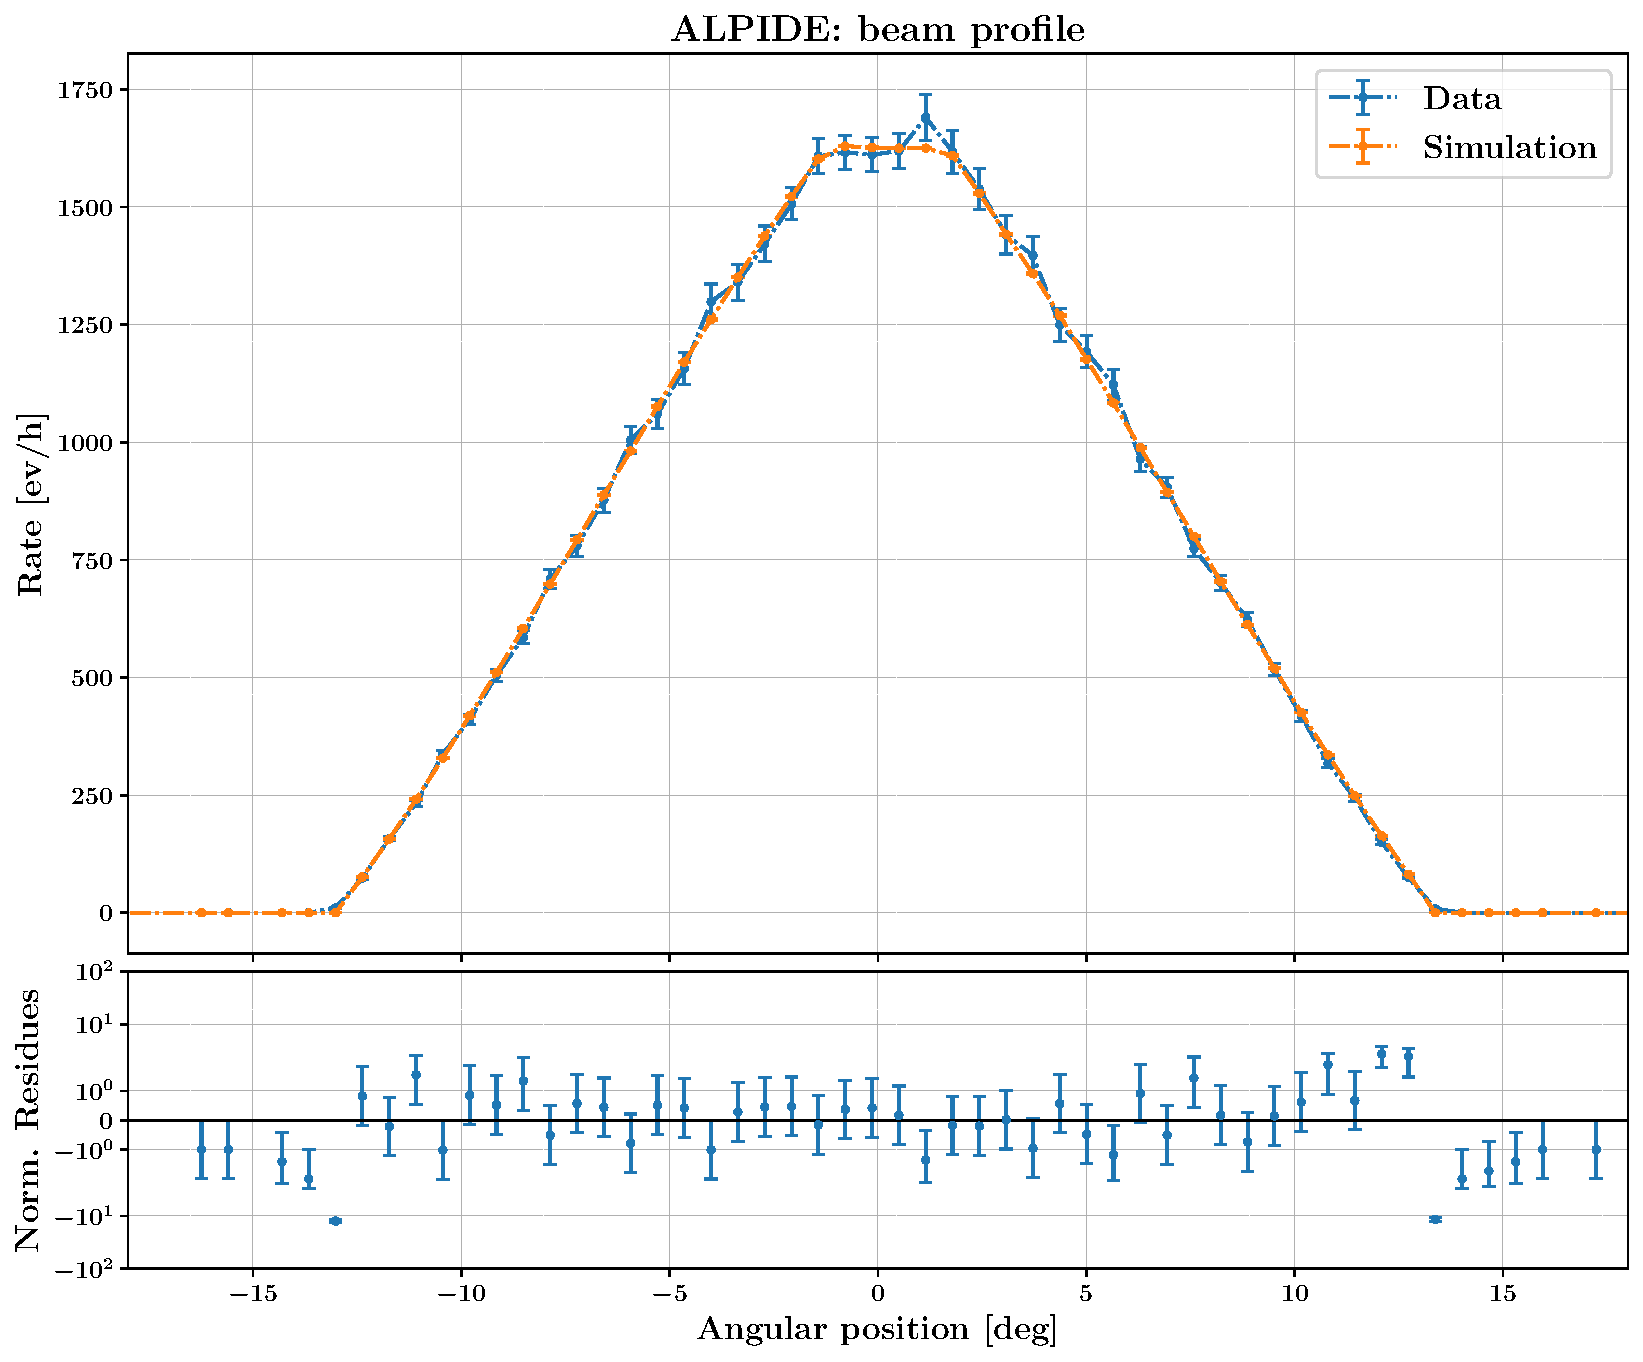
\includegraphics[height=6.5cm]{../sections/04/images/ALPIDE/ALPIDE_beam_profile.pdf}
            \label{fig:profile_ALPIDE}
        }
    \end{minipage}
    \caption{Beam profile comparison between the numerical simulation and the acquired spectrum with the SSB detector in \figref{fig:profile_picoscope} and with the ALPIDE detector in \figref{fig:profile_ALPIDE}.}
    \label{fig:profile}
\end{figure*}

\end{document}
